%!TeX root = thesis-main.tex
% The preceding line is only needed to identify funding in the first footnote. If that is unneeded, please comment it out.
%\usepackage[none]{hyphenat}


\theoremstyle{definition}
\newtheorem{example}{Example}
    
\newtheorem{theorem}{Theorem}
\chapter[Self-Organisation Programming]{
Self-Organisation Programming: A Functional Reactive Macro Approach
}
\minitoc% Creating an actual minitoc
%\begin{abstract}
%
%Engineering self-organising systems 
% -- e.g., robot swarms, collectives of wearables, or distributed infrastructures -- 
% has been investigated and addressed through
% various kinds of approaches: devising algorithms by taking inspiration from nature, relying on design patterns, using learning to synthesise behaviour from expectations of emergent behaviour, 
% and exposing key mechanisms and abstractions at the level of a programming language.
%
% Focussing on the latter approach, most of the state-of-the-art languages for self-organisation
%  leverage a round-based execution model,
%  where devices repeatedly evaluate their context and control program fully: this model is simple to reason about but limited in terms of flexibility and fine-grained management of sub-activities.
%
% By inspiration from the so-called functional reactive paradigm,
%  in this paper
%  we propose a \emph{reactive self-organisation programming approach}
%  that enables to fully decouple the program logic
%  from the scheduling of its sub-activities.
% 
% Specifically, we implement the idea
%  through a functional reactive implementation of aggregate programming in Scala, based on the functional reactive library Sodium.
%
% The result is a functional reactive self-organisation programming model, called \acs{langname}, that
%  maintains the same expressiveness and benefits of aggregate programming,
%  while enabling significant improvements in terms of scheduling controllability, flexibility in the sensing/actuation model, and execution efficiency. 
% \end{abstract}

% \begin{IEEEkeywords}
% self-organising systems,
% self-organisation programming,
% multi-agent systems, 
% emergent behaviour, 
% emergence steering, 
% functional reactive programming, 
% aggregate computing.
% \end{IEEEkeywords}

%\meta{Budget: 10 pages (incl. refs)}

Building \emph{artificial self-organising systems} 
 exhibiting \emph{collective intelligence}
 is a relevant research challenge 
 spanning science and engineering~\cite{DBLP:journals/ker/ParunakB15,gershenson2007design-sos,DBLP:conf/uksim/SinghSP13,DBLP:journals/sttt/NicolaJW20}.
%
A central problem lies in \emph{driving the (emergence of) self-organising behaviour
of a collection of agents or devices}---a goal also referred to through terms like
``guided self-organization''~\cite{prokopenko2009guided-selforg},
``controlled self-organization''~\cite{DBLP:journals/taas/SchmeckMCMR10}, and
``emergence steering''~\cite{Varenne2015morpho,DBLP:conf/sysose/Giammarco17a}.
%
This problem can be reduced to the definition of the control program
 that each agent has to execute~\cite{DBLP:journals/tib/MartiusH12}.
%
The problem can be addressed
 through \emph{automatic} approaches
(e.g., multi-agent reinforcement learning~\cite{DBLP:journals/corr/abs-1911-10635})
 or \emph{manual} approaches~\cite{DBLP:journals/tib/MartiusH12}
 based on the definition of control rules or 
 designs in terms of patterns involving, e.g.,
information flows and control loops~\cite{DBLP:conf/saso/WolfH07}.
%
Hybrid approaches are also possible where (parts of) programs
are generated or improved through learning~\cite{DBLP:conf/coordination/AguzziCV22}.

In this work, we focus on the \emph{programming language-based} approach to self-organization,
 where the developer writes the self-organising control program
 using a suitable \emph{macroprogramming language}~\cite{casadei2023macro,DBLP:journals/jisa/JuniorSBP21} (i.e., one aiming at expressing the macro-level behaviour of a system), be it general-purpose or domain-specific (e.g., explicitly tailored to robotic swarms~\cite{DBLP:journals/swarm/BrambillaFBD13} or wireless sensor networks~\cite{DBLP:journals/csur/MottolaP11}).
%
Specifically, our high-level goal
 is to devise a programming language
 for self-organising systems
 that is \emph{expressive}, \emph{practical},
 and \emph{declarative}---in the sense that it should allow the programmer to abstract from
many operational details, to be dealt with automatically by the underlying middleware/platform~\cite{DBLP:conf/iotdi/NoorTGS19,CPPVW-FI2020}.
%
Specifically, we focus on the problem of concrete scheduling of the sub-activities of which a self-organising system can be composed.
%
State-of-the-art languages typically leverage a \emph{round-based} execution model,
 where devices repeatedly evaluate their context and control program entirely
(typically in a loop or periodic, time-driven fashion).
%
This approach is simple to reason about but
 limited in terms of flexibility in scheduling
 and management of sub-activities (and response to contextual changes).
%
Motivated by this, and inspired by the functional reactive paradigm,
 in this work 
 \emph{we propose a reactive self-organization programming language
 that enables the decoupling of program logic from its scheduling}.
% 
In particular, as a contribution, we:
\begin{itemize}
\item propose a novel programming model and language, called \emph{\ac{langname}};
\item provide an open-source implementation as a Scala \ac{dsl}\footnote{\label{acsos2023-frp:footnote:dsl}\url{https://github.com/cric96/distributed-frp}},
 leveraging the functional reactive library Sodium and 
 inspiration from the \scafi{} aggregate programming \ac{dsl}~\cite{DBLP:journals/softx/CasadeiVAP22,DBLP:journals/lmcs/AudritoCDV23};
\item experimentally evaluate the benefits of reactivity and resource usage
through an open-source, permanently available artefact with reproducible simulations\footnote{\label{acsos2023-frp:footnote:eval}\url{https://github.com/AggregateComputing/experiment-2023-acsos-distributed-frp}}.
\end{itemize}
%
The result is a functional reactive self-organization programming model, 
 relying on functional composition of behaviours,
and whereby each sub-expression is amenable to independent scheduling:
 overall, we maintain the same expressiveness and benefits of aggregate programming~\cite{bpv:aggregate:programming,vbdacp:ac:survey:jlamp}
 while enabling significant improvements in terms of scheduling controllability, flexibility in the sensing/actuation model, and execution efficiency. %sec:contrib

%A relevant class of approaches
% is given by programming models
% where the developer specifies
% the control program of the agents
% of the system, which is scheduled
% in a time-driven or proactive way
% to sustain the self-organisation dynamics.
%%
%The typical computational model leverages 
% collections of devices,
% interacting with neighbours by exchanging messages,
% and working at synchronous or asynchronous
% sense--compute--interact rounds.
%%
%Similarly to natural systems,
% the self-organising behaviour
% of such systems 
% is based on the repetition of rounds involving three main steps: 
% context assessment (e.g., reading sensors and collecting messages from neighbours),
% decision-making (i.e., evaluation of a program against the current context),
% and interaction (e.g., running actuators and sending messages to neighbours).
%
%The model abstracts from the scheduling of rounds: concrete policies are application-specific, and may be time-driven, reactive, or based on learned heuristics.
%
%However, often 
% rounds are considered atomically,
% which means that all the possible source of changes are continuously considered,
% and it is not possible to perform fine-grained scheduling of parts of the control program---which would be desirable to make collective computations more time- and energy-efficient.

The rest of the article is organized as follows.
%
\Cref{acsos2023-frp:sec:background} covers background on self-organization programming and the functional reactive paradigm.
%
\Cref{acsos2023-frp:sec:contrib} presents the \ac{langname} programming model.
%
\Cref{acsos2023-frp:sec:impl} details the implementation.
%
\Cref{acsos2023-frp:sec:eval} describes the experimental setup and results.
%
\Cref{acsos2023-frp:sec:conc} draws conclusions and future research work.
 
\section{Background and Motivation}\label{acsos2023-frp:sec:background}

%\meta{
%budget: 1 pages
%}

In this section,
 we review approaches for self-organization engineering (\Cref{acsos2023-frp:sec:background:selforg}),
 and set the goal of combining the benefits of reactive approaches
with those of compositional macroprogramming models like aggregate computing.
%
Then, we provide background on \ac{frp} (\Cref{acsos2023-frp:sec:background:frp}),
 the paradigm we choose for our programming model,
 for its benefits in declarativity and
 automatic, configurable management of change.

\subsection{Self-organization Engineering Approaches}
\label{acsos2023-frp:sec:background:selforg}

%\section{Related Work}

%\meta{Plan: we may briefly recall the kinds of approaches as per the Intro. And then cover a few approaches for programming self-org, such as: TOTA as representative for reactive models, and AC as representative for proactive models?}

The first distinction in approaches for self-organization engineering
 is between automatic 
 and manual approaches.
%
In the former category, 
 the control logic of the agents
 is learned, synthesized, or evolved automatically---as e.g., in multi-agent reinforcement learning~\cite{DBLP:journals/corr/abs-1911-10635},
 Collective Intelligence~\cite{tumer2004collectives,casadei2023artl-ci-survey},
 and evolutionary swarm robotics~\cite{trianni2008evolutionary-swarm}.
%
The latter category, instead,
 involves explicit engineering of the activity
 by a developer,
 e.g., by reusing patterns of behaviour~\cite{FDMVA-NACO2013}, by directly coding the individual logic of each type of device,
 or by using mechanisms provided by a so-called \emph{macroprogramming language}\cite{casadei2023macro,DBLP:journals/jisa/JuniorSBP21}.
%
The rest of the section covers prominent approaches in this category (i.e.\ programming models)---distinguishing between reactive and round-based ones.

Among reactive approaches is \emph{Tuples On The Air (TOTA)}~\cite{tota},
 a programming model for decentralized peer-to-peer networks of mobile nodes or agents.
%
It uses \emph{tuples} to represent context information 
 and mediate interactions between agents.
%
In particular, tuples are \emph{reactive}: they are associated with propagation rules that
describe how tuples should be propagated to neighbours (hop-by-hop) in a network and how the
content of tuples should change during propagation
 or in reaction to environmental events. 
%
The agents behave and coordinate
 through operations on tuples (e.g., insertion, read, removal, waiting) or by subscribing to tuple-related events.
%
Other reactive approaches exist, such as the \emph{Higher-Order Chemical Language (HOCL)}\cite{DBLP:journals/ijuc/BanatreFR07},
 but they feature quite a large abstraction gap.
%% HOCL =
%% supports expressing self-organising computations
%% in terms of chemical solutions
%% consisting of \emph{molecules} (data) interacting according to \emph{reactive rules}.
%

On the other side, there are programming models 
 based on a \emph{round-based} execution model
 whereby 
 each device repeatedly performs a complete evaluation of its control program
 (e.g., wrapped in a loop or scheduled in a periodic, time-driven fashion).
%  involved in \emph{sense--compute--interact} rounds, scheduled in a time-driven fashion,
% and the languages provide a convenient way to express the \emph{compute} step, which typically involves the overall self-organising system to be executed.
%
Aggregate computing~\cite{bpv:aggregate:programming,vbdacp:ac:survey:jlamp}
is one such approach,
  where each round is atomically composed of \emph{sense--compute--interact} steps,
  and a language is used to express the \emph{compute} step conveniently.
%
Indeed, it emerged as 
 a prominent approach for programming
 self-organization~\cite{vbdacp:ac:survey:jlamp},
 with the benefits of formality,
 abstraction, compositionality, and pragmatism.
%
Formality stems from building the approach
 over \emph{field calculi}~\cite{vbdacp:ac:survey:jlamp} with well-defined language semantics.
%
Abstraction comes from the declarativity of the \emph{functional} programming model,
 promoting different scheduling strategies~\cite{DBLP:conf/acsos/AguzziCV22,DBLP:journals/lmcs/PianiniCVMZ21} 
 and deployments~\cite{CPPVW-FI2020}, possibly applied automatically to different sub-activities concurrently running.
%
Compositionality comes from adopting the functional paradigm and the \emph{field abstraction}~\cite{DBLP:journals/pervasive/MameiZL04,vbdacp:ac:survey:jlamp}
(a field is a map from a domain of devices to computational values---e.g., a field of temperatures, or a field of velocity vectors).
%
Finally,
pragmatism is supported by the language design and its separation of concerns,
 which enables modular \acp{dsl} and toolkits~\cite{DBLP:journals/softx/CasadeiVAP22}.

Though conceptually simple,
 the round-based models could be more efficient,
 because they fully re-evaluate the context
 and the whole program
 without tracking change.
%
Though it might be acceptable for predictable patterns of environmental change,
  this becomes largely suboptimal for highly variable dynamics.
%
Indeed,
the round-based approach seems to be a legacy of imperative languages or solutions featuring limited compositionality.
Instead, more compositional languages like, e.g., aggregate computing languages~\cite{vbdacp:ac:survey:jlamp,DBLP:journals/nca/BachrachBM10,DBLP:conf/ecoop/AudritoCDSV22} and Buzz~\cite{DBLP:conf/iros/PinciroliB16},
 allow building complex self-organising behaviour
 by composing \emph{blocks} of simpler self-organising behaviours---see \Cref{acsos2023-frp:paradigmatic-examples} for examples.
% reactivity also makes sense for self-organisation,
% because the idea is to steer behaviour
% as a response to (local) change.
%
Therefore, each individual block of behaviour 
  is \emph{potentially independent of others (i.e., independently schedulable)},
  with data dependencies arising from each composition.
%
A reactive extension of aggregate computing has been proposed in~\cite{DBLP:journals/lmcs/PianiniCVMZ21},
  based on manually specifying dependencies and reactive policies (with configurable triggers) among different aggregate computations.
%
Instead,
a more practical approach could be
decoupling programs from the specification of reactive policies
and letting them only define the data dependencies between program portions.
%
The most suitable programming approach for this
 is the \emph{functional reactive programming} paradigm~\cite{DBLP:journals/csur/BainomugishaCCMM13}, briefly introduced in the following.
%
%\meta{RC: we might provide a table to show the pros \& cons of the discussed reactive and proactive approaches}
%\meta{MV: possibly, not strictly needed I feel}

\subsection{Functional Reactive Programming}
\label{acsos2023-frp:sec:background:frp}

\emph{Reactive programming}~\cite{DBLP:journals/csur/BainomugishaCCMM13} is a paradigm suitable for developing event-driven applications,
 leveraging abstractions to express (relationships between) time-varying values and 
 automatically handle the propagation of change
(cf.\ the paradigmatic example of spreadsheets~\cite{blackheath2016frp-sodium}).
%
%It is very much related to the \emph{synchronous dataflow programming} paradigm~\cite{DBLP:journals/pieee/LeeM87} for concurrent/parallel systems.
%
Reactive programming is often combined with the functional programming paradigm~\cite{DBLP:journals/csur/BainomugishaCCMM13,blackheath2016frp-sodium}
in the so-called \ac{frp}.

\newcommand{\Time}{\ensuremath{\mathit{Time}}}
\newcommand{\Sg}{\ensuremath{\mathit{Cell}}}
\newcommand{\St}{\ensuremath{\mathit{Stream}}}

\Ac{frp} builds on few abstractions and various combinators~\cite{DBLP:conf/pldi/WanH00}.
%
Conceptually,
\ac{frp} considers \emph{continuous time}, $\Time = \{ t \in \mathbb{R} \mid t \geq 0 \}$.
%
Time-varying values are called \emph{cells}
 and may be conceptually modelled by generic functions of type $\Sg\:a: \Time \to a$.
%
Then, \emph{streams} are discrete-time values
 and may be modelled by generic functions of type
$\St\:a: [\Time] \to [a]$ (where notation $[X]$ indicates sequences of $X$s), namely, 
mapping a sequence of (increasing) sample times to a sequence of corresponding values.
%
While cells model state,
 streams model state changes (or events).
%
Then, \ac{frp} libraries %languages
 provide functions (combinators) for transforming signals to signals,
  streams to streams,
  signals to streams,
  and streams to signals.
%
An example of such a library %  language 
 is Sodium~\cite{blackheath2016frp-sodium},
 the Java library for \ac{frp}
 which we leveraged to implement \ac{langname} as described in \Cref{acsos2023-frp:sec:impl}.
  
%To more practically introduce \ac{frp}, in the following we briefly recap the essential elements of Sodium~\cite{blackheath2016frp-sodium},
% a Java library for \ac{frp}
% which we leveraged for the implementation of \ac{langname} as described in \Cref{acsos2023-frp:sec:impl}.

 

\paragraph*{Background: Sodium}
Sodium is primarily based on two types:
%
\begin{itemize}
  \item \texttt{Cell<T>} represents a value of type \texttt{T} that changes over time;
  \item \texttt{Stream<T>} represents a sequence of emissions of events, each holding data of type \texttt{T}.
\end{itemize}
%
In addition, Sodium implements a series of \textit{primitives} that can be used to perform transformations on cells and streams. 

\paragraph{Never}
A stream that will never emit any events can be created by using the empty constructor of \texttt{Stream<T>}:
%
\begin{lstlisting}[frame=single, language=java]
Stream<String> never = new Stream<>();
\end{lstlisting}

\paragraph{Constant}
A cell that will always have the given value can be created by passing a constant value to the constructor of \texttt{Cell<T>}:
%
\begin{lstlisting}[frame=single, language=java]
Cell<String> helloWorld = new Cell<>("Hello World!");
\end{lstlisting}


\paragraph{Map}
A stream (resp. cell) can be transformed into a corresponding stream (resp. cell) through method  \texttt{x.map(f)}, where \texttt{f} is the mapping function:
%
\begin{lstlisting}[frame=single, language=java]
Stream<Integer> source = ...;
Stream<String> out = source.map(x -> Integer.toString(x));

Cell<Integer> source = ...;
Cell<String> out = source.map(x -> Integer.toString(x));
\end{lstlisting}  

%\paragraph{Map (cell)}
%Produces a cell whose value is taken from the source cell by applying a mapping function.
%%
%\begin{lstlisting}[frame=single, language=java]
%Cell<Integer> source = ...;
%Cell<String> out = source.map(x -> Integer.toString(x));
%\end{lstlisting}

\paragraph{Merge}
Two streams of the same type can be merged into a single stream via the \texttt{s1.merge(s2,f)} method,
 where a mapping function \texttt{f} can be used to combine \emph{simultaneous events}. 
%, returning a stream that emits events from either input.
%
%Since Sodium supports \textit{simultaneous events} (see \Cref{acsos2023-frp:sec:transactions} for more details), if both input streams happen to emit at the same time the given combining function will be used to produce the final output event.
%
\begin{lstlisting}[frame=single, language=java]
Stream<Integer> left = ...;
Stream<Integer> right = ...;
Stream<Integer> merged = left.merge(right, (l, r) -> l + r);
\end{lstlisting}

\paragraph{Hold}
A stream \texttt{s} can be converted into a cell through method \texttt{s.hold(init)}: the cell, holding \texttt{init} before the first event, will keep the value of the most recent event.
%
\begin{lstlisting}[frame=single, language=java]
Stream<Integer> events = ...;
Cell<Integer> hold = events.hold(0);
\end{lstlisting}

\paragraph{Snapshot}
A cell can be converted into a stream
 through method \texttt{s.snapshot(c,f)}:
 the output stream will capture the values of the given cell \texttt{c} whenever the source stream \texttt{s} fires.
%
%Produces a stream firing at the same time as the source stream and emitting combinations of the values from the stream and the cell using the supplied function.
%
\begin{lstlisting}[frame=single, language=java]
Stream<String> trigger = ...;
Cell<Integer> state = ...;
Stream<String> out = trigger.snapshot(state, (t, s) -> t + s);
\end{lstlisting}

\paragraph{Filter}
Method \texttt{s.filter(f)} produces a stream that emits only the events from the source stream \texttt{s} that satisfy the given predicate \texttt{f}.
%
\begin{lstlisting}[frame=single, language=java]
Stream<Integer> events = ...;
Stream<Integer> out = events.filter(x -> x > 0);
\end{lstlisting}

\paragraph{Lift}
Two cells can be combined into one through a method \texttt{c1.lift(c2,f)}, where \texttt{f} is a combining function.
%
\begin{lstlisting}[frame=single, language=java]
Cell<Integer> left = ...;
Cell<Integer> right = ...;
Cell<Integer> out = left.lift(right, (l, r) -> l + r);
\end{lstlisting}

\paragraph{Sample}
The sampling of a cell returns the current value wrapped by the cell.
%
\begin{lstlisting}[frame=single, language=java]
Cell<String> state = ...;
String currentState = state.sample();
\end{lstlisting}
  
\paragraph{Switch (stream)}
Flattens a cell of streams into a single stream that emits whenever the active stream for the cell emits.
%
\begin{lstlisting}[frame=single, language=java]
Cell<Stream<Integer>> source = ...;
Stream<Integer> out = Cell.switchS(source);
\end{lstlisting}
%
\paragraph{Switch (cell)}
Flattens a cell of cells into a single cell whose value is the value of the active cell of the wrapper cell.
\begin{lstlisting}[frame=single, language=java]
Cell<Cell<Integer>> source = ...;
Cell<Integer> out = Cell.switchC(source);
\end{lstlisting}

%\meta{\texttt{CellLoop<T>}?}
  
Combining streams and cells yields a directed graph across which changes propagate
that forms a piece of functional reactive logic.
%
External interfacing with \ac{frp} graphs
 is supported by
 (i) \emph{pushing events into streams and cells}, by leveraging types \texttt{StreamSink<T>} and \texttt{CellSink<T>};
 and
 (ii) \emph{listening to changes in streams and cells}, through method \texttt{listen(h)} attaching handler \texttt{h}.
 
\section{The \ac{langname} Programming Model}
\label{acsos2023-frp:sec:contrib}

%\meta{
%budget: 2,5/3 pages
%
%SECTION IDEA/NARRATIVE: explain the programming model by a user point of view (like a tutorial)
%}

This section presents the \ac{langname} programming model from a user perspective.
%
First, we explain the system and execution model (\Cref{acsos2023-frp:sec:sys-model});
 then, we present the language abstractions and primitives (\Cref{acsos2023-frp:programming-constructs});
 finally, we show how paradigmatic examples of self-organization can be expressed in \ac{langname} (\Cref{acsos2023-frp:paradigmatic-examples}).

\subsection{System Model and (Reactive) Execution Model}
\label{acsos2023-frp:sec:sys-model}

%\meta{devices, sensors, actuators, neighborhoods
%
%NEED TO explain the execution model which is driven reactively from changes in the context (explain that context is given by msgs, sensors, etc.)
%}

We shall program the self-organising behaviour of a \emph{system} of \emph{devices}.
%
A \emph{device} 
 has a \emph{unique identifier (ID)},
 as well as
 \emph{sensors} and \emph{actuators}
 that allow it to perceive and act upon its surrounding \emph{environment}.
%
A device can interact with other devices (its \emph{neighbours}, forming a dynamic set)
 by exchanging messages asynchronously.
%
A device has an associated \emph{program}
 that defines its behaviour.

The program that a device runs
 can be defined compositionally, and it
 generally computes over
 its \emph{local context},
 which consists of 
 (i) a sampling of its sensor values
 and 
 (ii) the data provided by neighbours through messages.
%
Without loss of generality, we assume that all the data provided by a neighbour is consolidated into a single object
(i.e., \emph{one object per neighbour})
and that neighbour data may \emph{expire}
(i.e., it may be set to be valid for a configurable, limited lifetime).
%
The execution of a program (computation) provides an \emph{output} object
 and defines what data has to be packed into a message, also called an \emph{export}, to be sent to all the neighbours.
%
The export can be thought of as an associative map of keys and values,
where keys denote different sub-computations and values the data relevant to those sub-computations.

In general, the \emph{scheduling} of a program execution 
is asynchronous w.r.t.\ other devices
  and may be periodic (time-triggered)
  or reactive.
%
In this work, we consider reactive scheduling
and compare it with the periodic scheduling of earlier research.
%
In reactive settings, 
 a program may need to be re-executed any time an input changes, i.e.:
%
\begin{itemize}
\item sensor data (e.g., the temperature sensor perceives a different temperature);
\item neighbour data
    (e.g., a device is no longer a neighbour,
    a message has expired,
    or a neighbour provides a more recent message that supersedes previous data).
\end{itemize}
%
A re-evaluation of the program
 may produce a different output and export.  
%
Furthermore, 
 in this work, we take this reactivity scheduling of programs a step further
 by allowing individual \emph{expressions} (i.e., portions of programs)
 to be re-evaluated when their context and inputs (e.g., dependencies on other expressions) change---thanks to the \ac{frp} approach.
%
This idea will be shown in \Cref{acsos2023-frp:ex:channel} and \Cref{acsos2023-frp:fig:channel:graph}.

Notice that the model is logical 
 and may be implemented using different approaches and optimizations---e.g., a device may send a heartbeat to notify that it is still a neighbour and its data has not changed,
 it may send a message with only data that has changed, and so on.
%
Also, inbound and outbound reactivity can be regulated by throttling, i.e.,
 by accumulating a certain amount of (change in) inputs (before re-evaluating the program or parts of it)
 and  accumulating a certain amount of (change in) outputs/exports
 (before executing actuations and/or sending the export to neighbours).
 
%
%\meta{RC: can we provide a picture of the idea?}

\subsection{Programming Abstractions and Primitives}
\label{acsos2023-frp:programming-constructs}

%\meta{rep/LOOP, nbr, branch-- introduced through simple examples (see e.g. the progression of examples from~\cite{DBLP:journals/lmcs/AudritoCDV23}: counting rounds (here, we should provide a frequency explicitly), counting the number of neighbours or getting the mean of a value from neighbourhood}

We adopt a \emph{macroprogramming} approach\cite{casadei2023macro},
 where a single program
 is used to express the collective behaviour
 of the entire system of devices.
%
Specifically,
 the self-organising collective behaviour
 will \emph{emerge}
 from 
 (i) the local execution of the program
 by all the devices making up the system, 
 (ii) the distributed execution (implementing the message passing),
 and 
 (iii) the environment dynamics (which will affect neighbourhoods and the data perceived by sensors).

%
%All the constructs of the \texttt{Language} deal with \texttt{Flow}s, a type which is designed to encapsulate aggregate (sub-)computations as a dependency graph (in a way that's closely related to the dependency graph of an FRP engine).
%%
%A \texttt{Flow} is essentially a function that takes a path and a \texttt{Context} and returns a cell of \texttt{Export}s, possibly depending on the exports of other \texttt{Flow}s recursively.
%%
%The path represents the point in the evaluation tree where that \texttt{Flow} is placed, while the \texttt{Context} places the computation inside some device.

Since \ac{langname} is implemented as a \ac{dsl} internal (or embedded) in Scala,
 Scala types and features (e.g., functions)
 can be reused in \ac{langname} programs.

\subsubsection{Datatypes}
%
According to the \ac{frp} paradigm,
 we would like to express
 a self-organising collective computation
 as a graph of reactive sub-computations.
%
We call each sub-computation a \emph{flow}
 and represent it programmatically through type \lstinline|Flow[T]|\footnote{Notation: we highlight types in {\color{brown!50!black}\texttt{brown}}, primitives in {\color{red}\texttt{red}}, derived/library constructs in {\color{purple}\texttt{purple}}, and Scala (host language) keywords in {\color{blue}\textbf{\texttt{blue}}}.}, where \lstinline|T| is the type of the output of the wrapped computation.
%
A \lstinline|Flow| is essentially a function that takes %a path and 
a \lstinline|Context| and returns a \emph{cell} of \lstinline|Export|s, possibly depending on the exports of other \lstinline|Flow|s, recursively---see \Cref{acsos2023-frp:sec:impl:impl} for details.
%
With abuse of terminology,
 we will refer to a flow 
 as its output cell, i.e., as a time-varying value.

\subsubsection{Local values}
%
The simplest constructs of the language are local and atomic 
(i.e., that do not depend on other flows or neighbours).
%
%Being atomic, their corresponding trees only contain a root node with the final value of the expression:
\begin{itemize}
    \item \lstinline|constant(e)| returns a constant flow that always evaluates to the argument that has been passed;
    \item \lstinline|sensor(name)| returns the flow of values produced by the sensor with the given \texttt{name};
    %implements the sensing abilities of each device uses the cell returned by the \texttt{Context} for the given sensor name;
    \item \lstinline|mid()|, as a shortcut to \lstinline|sensor("mid")|, returns the constant flow of the device ID. %s always evaluates to the \texttt{selfId} returned by the \texttt{Context};
\end{itemize}


\subsubsection{Choice}
%
A \lstinline|mux(c){t}{e}| expression
 returns a flow with the same output of flow \texttt{t} when the Boolean flow \texttt{c} is true and the output of flow \texttt{e} when \texttt{c} is false.
%
E.g., code 
\begin{lstlisting}
mux(sensor("temperature") > THRESHOLD)
    { constant("hot") } { constant("normal") }
\end{lstlisting}
will yield the string \lstinline|"hot"|
in the devices where the local temperature sensor yields a value below the given threshold
and the string \lstinline|"normal"| otherwise.

%(\Cref{acsos2023-frp:fig:semantics-mux}) is an alternative to \texttt{branch} that introduces conditional behaviour without resulting in partitions in the device network.
%
%That is, devices running sub-computations in \texttt{t} or \texttt{e} will always align with each other since both exports will be included in the final one, respectively under the \texttt{Then} and \texttt{Else} slots.

%
%\begin{figure}
%    \centering
%    \begin{subfigure}[b]{0.47\textwidth}
%        \centering
%        \includegraphics[width=\textwidth]{figures/semantics/mux-true.pdf}
%        \caption{\texttt{true} condition.}
%        \label{acsos2023-frp:fig:semantics-mux-true}
%    \end{subfigure}
%    \begin{subfigure}[b]{0.47\textwidth}
%        \centering
%        \includegraphics[width=\textwidth]{figures/semantics/mux-false.pdf}
%        \caption{\texttt{false} condition.}
%        \label{acsos2023-frp:fig:semantics-mux-false}
%    \end{subfigure}
%    \caption{Semantics of \texttt{mux(c, t, e)}.}
%    \label{acsos2023-frp:fig:semantics-mux}
%\end{figure}

\subsubsection{Interaction with neighbours}
%
Communication with neighbours is handled \emph{in both directions at once} through a single construct, \lstinline|nbr(f)|, which takes a flow \texttt{f} as parameter.
%
The local output of \texttt{f} will be automatically sent to neighbours.
%
Instead, the output of the whole \lstinline|nbr(f)| expression
 is an object \lstinline|NeighborField[T]|
 collecting the values of \texttt{f} computed by all the neighbours.
%
For instance
%
\begin{lstlisting}
nbr(mid()) // or nbr(mid()).withoutSelf to exclude "self"
\end{lstlisting}
%
returns, in any device, the IDs of all its neighbours (including the device itself).
%
%Neighbouring constructs, i.e., \texttt{nbr} and \texttt{nbrSensor}, require knowing which neighbours are aligned when they get evaluated. %, as shown in \Cref{acsos2023-frp:fig:semantics-neighboring}.
%
%This means that, if this constructs are used at a certain path \texttt{p}, the engine should filter out all neighbours whose known export does not contain \texttt{p}.
%%
%Furthermore, only the sub-exports rooted at \texttt{p} of each neighbour need to be considered.
%
%The \texttt{nbr(a)} constructs works by collecting all neighbouring values of \texttt{a}. %, which can be found at \texttt{p / Nbr} for each neighbour.
%
%Since every device is a neighbour of itself, this process should also take care of replacing the value produced by the previous evaluation with the new value coming from \texttt{a}.
%
%This is shown in \Cref{acsos2023-frp:fig:semantics-nbr} by the isolated arrow going from \texttt{r(a)} in the current device to the root of the export.
%
%For what concerns \texttt{nbrSensor}, the engine just uses the current \texttt{NeighborState} of each aligned neighbour to evaluate the sensor with the specified identifier.

Sensors providing a value for each neighbour have dedicated syntax.
%
They can be queried through construct \lstinline|nbrSensor(name)|.
%
For instance,
the built-in function \lstinline|nbrRange|, defined as follows:
\begin{lstlisting}
def nbrRange(): Flow[NeighborField[Double]] = 
  nbrSensor("nbrRange")
\end{lstlisting}
provides the neighbouring field of (estimated) distances to neighbours
(how such a sensor works is an implementation detail---e.g., it may use GPS traces or Wi-Fi signal strength).
%
%\begin{figure}
%    \centering
%    \begin{subfigure}[b]{0.47\textwidth}
%        \centering
%        \includegraphics[width=\textwidth]{figures/semantics/nbr.pdf}
%        \caption{\texttt{nbr(a)}}
%        \label{acsos2023-frp:fig:semantics-nbr}
%    \end{subfigure}
%    \hfill
%    \begin{subfigure}[b]{0.47\textwidth}
%        \centering
%        \includegraphics[width=\textwidth]{figures/semantics/nbrSensor.pdf}
%        \caption{\texttt{nbrSensor(s)}}
%        \label{acsos2023-frp:fig:semantics-nbrsensor}
%    \end{subfigure}
%    \caption{Semantics of neighboring constructs.}
%    \label{acsos2023-frp:fig:semantics-neighboring}
%\end{figure}



\subsubsection{Branching}
%
An expression \lstinline|branch(c){t}{e}|
evaluates and returns the value of expression \texttt{t} (resp. \texttt{e})
when \texttt{c} evaluates to \lstinline|true| (resp. \lstinline|false|).
 % only the export selected by \texttt{c} is included in the final output.
%
%In cases where the condition is true, \texttt{t} is included under the \texttt{Then} slot and its root is used as the global root, otherwise \texttt{e} is included under the \texttt{Else} slot and its root is used instead.
%%
%In both cases, \texttt{c} is inserted under the \texttt{Condition} slot.
%
This enables a form of distributed branching,
where devices that happen to execute \texttt{t}
will not interact with those that executed \texttt{e} (and vice versa)---unlike \lstinline|mux| in which a device ``contributes'' to both \texttt{t} and \texttt{e}.
%
E.g.,
in a system split into red and blue devices, the expression:
\begin{lstlisting}
branch(sensor("color") == "red"){
  nbr(constant(1)).sum // red nodes run this
} { 
  nbr(constant(1)).sum // blue nodes run this
}
\end{lstlisting}
will yield in any device the number of neighbours \emph{of the same kind},
neighbours that run the other sub-computation
(despite those being the same) will not be considered.
%
This concept is called \emph{alignment} and is well-discussed, e.g., in~\cite{DBLP:journals/lmcs/AudritoCDV23}.
% 
Notice that, upon a change in the value sensed by \texttt{colour},
 a device may dynamically switch branch and hence sub-computation domain and ``aligned'' neighbour set.
 
%With this semantics, any sub-computation under \texttt{t} or \texttt{e} will not align with any neighbor executing the opposite branch. %, due to the fact that their paths will differ at the \texttt{Then}/\texttt{Else} slot.
%
%\begin{figure}
%    \centering
%    \begin{subfigure}[b]{0.40\textwidth}
%        \centering
%        \includegraphics[width=\textwidth]{figures/semantics/branch-true.pdf}
%        \caption{\texttt{true} condition.}
%        \label{acsos2023-frp:fig:semantics-branch-true}
%    \end{subfigure}
%    \begin{subfigure}[b]{0.40\textwidth}
%        \centering
%        \includegraphics[width=\textwidth]{figures/semantics/branch-false.pdf}
%        \caption{\texttt{false} condition.}
%        \label{acsos2023-frp:fig:semantics-branch-false}
%    \end{subfigure}
%    \caption{Semantics of \texttt{branch(c, t, e)}.}
%    \label{acsos2023-frp:fig:semantics-branch}
%\end{figure}


\subsubsection{Lifting} 
%The language also defines a \texttt{lift} construct.
%%
%\textit{Lifting} is a well-known concept of functional programming that allows a function working with atomic values to be applied to wrapped versions of those values, for some wrapper type.
%%
%In this case, the wrapper type is the \texttt{Flow} type, and lifting a function to the \texttt{Flow} world means producing another \texttt{Flow} obtained by applying that function to the roots of those flows, and having the original exports as children of the resulting one.
%
%This is shown in \Cref{acsos2023-frp:fig:semantics-lift}, which depicts the case where \texttt{f} is a binary function (the generalization to n-ary functions is in fact trivial).
%
%\begin{figure}
%    \centering
%    \includegraphics[width=0.4\textwidth]{figures/semantics/lift.pdf}
%    \caption{Semantics of \texttt{lift(a, b, f)}.}
%    \label{acsos2023-frp:fig:semantics-lift}
%\end{figure}
%As a side note, the specification also defines a \texttt{lift} operation on instances of \texttt{NeighborField}s.
%%
%It has the effect of evaluating the given function on pairs of values associated with the same device and returning the outputs as another \texttt{NeighborField}.
%
Lifting enables flow combination: i.e.,
 \lstinline|lift(f1,f2,...,fN){g}|
 yields a flow obtained by applying \texttt{g(o1,o2,...,oN)} where \texttt{o\emph{i}} is the output of flow \texttt{f\emph{i}}.
%
Lifting can also be applied on flows of \lstinline|NeighborField|s,
in which case
the output is a flow of a \lstinline|NeighborField|
whose values are combined from the input \lstinline|NeighborField|s neighbour-wise (runtime checks avoid combining flows with different domains).
%
E.g.,
\begin{lstlisting}
lift(nbr(mid(),nbrRange()){(nbrId,nbrDist) =>
  s"${nbrId} is at distance ${nbrDist} from me"}
\end{lstlisting}
%
yields locally to a device one string per neighbour reporting its ID and distance.

\subsubsection{Looping (state evolution)}
%The final construct is \texttt{loop}.
%
%This is designed to be an adaptation of \texttt{rep} as defined by field calculus to the reactive model.
%
%This change was necessary due to the fact that \texttt{rep} is based on the underlying execution model structured in computation rounds, but that's not the case in the reactive model.
%
%Instead of using proactive and repeated application of a function,
% 
Construct \lstinline|loop(init,ft)| evolves a piece of state
(initially, \texttt{init})
 by applying function \texttt{ft} mapping the
previous state's flow to the next state's flow.
%
For instance, the expression:
%
\begin{lstlisting}
loop(0)(v => v + 1)
\end{lstlisting}
%
represents a computation counting from $0$ onwards (ignoring overflow).
%
How frequently does this counting progress?
%
It depends on the implementation of \lstinline|Context|,
  which provides a default throttling period.
%
A different \lstinline|loop| implementation may also accept a stream
explicitly dictating the pace of the stateful computation
(e.g., evolving state each time a button is pressed).

%
%Other than the initial state, \texttt{loop} accepts a function transforming a \texttt{Flow} into another \texttt{Flow} of the same type.
%%
%These \texttt{Flow}s shall be interpreted as the input always being \quotes{one step behind} the output.
%%
%The specification states that the \quotes{off-by-one} \texttt{Flow} should be constructed by aligning with the previous state of the same device, which can be read from the context leveraging the fact that every device is a neighbor of itself. % (\Cref{acsos2023-frp:fig:semantics-loop-next}).
%%
%In cases where alignment is not possible (i.e., on the first evaluation or after a switch of branch), the first argument of loop should be used to construct a new export. % (\Cref{acsos2023-frp:fig:semantics-loop-init}).
%%
%The implementation should take care of the following caveats arising from the intrinsic self-dependency of \texttt{loop}:
%%
%\begin{itemize}
%    \item \textit{infinite recursion}: since computations are triggered by themselves changing in the past, \texttt{loop} should not cause \textit{stack overflows} and therefore should use some sort of \textit{rate-limiting} strategy (e.g., \textit{throttling});
%    \item \textit{indefinite export growth}: a flow defined in terms of itself might cause the export tree to grow on each update, since exports are repeatedly wrapped in other exports; the implementation should take care of passing an \textit{atomic} flow as an input to the subsequent computation, in order to avoid indefinite growth.
%\end{itemize}
%
%\begin{figure}
%    \centering
%    \begin{subfigure}[b]{0.47\textwidth}
%        \centering
%        \includegraphics[width=\textwidth]{figures/semantics/loop-init.pdf}
%        \caption{Not aligned with previous state}
%        \label{acsos2023-frp:fig:semantics-loop-init}
%    \end{subfigure}
%    \hfill
%    \begin{subfigure}[b]{0.47\textwidth}
%        \centering
%        \includegraphics[width=\textwidth]{figures/semantics/loop-next.pdf}
%        \caption{Aligned with previous state}
%        \label{acsos2023-frp:fig:semantics-loop-next}
%    \end{subfigure}
%    \caption{Semantics of \texttt{loop(i, f)}.}
%    \label{acsos2023-frp:fig:semantics-loop}
%\end{figure}


\subsection{Paradigmatic Examples: Self-Healing Gradient \& Channel}
\label{acsos2023-frp:paradigmatic-examples}

In this section, we cover two fundamental self-organising behaviours
that will be exercised in the evaluation in \Cref{acsos2023-frp:sec:eval}.
%
Firstly, we introduce the \emph{gradient}~\cite{DBLP:conf/ipsn/NagpalSB03,audrito2017ULT}, a versatile
 self-organization pattern
 that supports a wide range of more complex self-organising behaviours.
%

\begin{example}[Self-Healing Gradient]\label{acsos2023-frp:ex:g}
%
A \emph{(self-healing) gradient} is a distributed behaviour 
 that \emph{self-stabilises}~\cite{dolev}, in each device  of the distributed system, 
 to a value denoting its minimum distance
 from the closest \emph{source} node (e.g., computed by summing the neighbour-to-neighbour distances along the shortest path to the source),
 adapting to changes in the source set and distances.
%
By following the neighbours of maximum decrease (resp. increase) of the gradient value, i.e., by descending (resp. ascending) the gradient,
 it is possible to implement efficient hop-by-hop information flows~\cite{DBLP:conf/saso/WolfH07},  e.g., useful for data propagation and collection.
%
%
%It generally takes multiple rounds to stabilise.
%%
%A \emph{self-healing} gradient can correct the collective output after a change in its inputs (i.e., the source set and the distances).
%
\Cref{acsos2023-frp:fig:scenario-g} provides a representation of a gradient.
 
Multiple gradient computation algorithms exist~\cite{audrito2017ULT}. A basic algorithm can be implemented in \ac{langname} as follows.

\begin{lstlisting}
def gradient(source: Flow[Boolean]): Flow[Double] =
  loop(Double.PositiveInfinity) { g => {
    mux(source) {
      constant(0.0)
    } {
      lift(nbrRange(), nbr(g)){_ + _}
        .withoutSelf
        .min
    }
  }
\end{lstlisting}
%
The function takes the Boolean \lstinline|source| flow as input, denoting whether the executing node is the source of the gradient or not.
%
The external \lstinline|loop| is used to progressively evolve the current gradient value \lstinline|g|
starting from an infinite value
(as, initially, we do not know whether a source is reachable).
%
Internally to the loop,
  we use \lstinline|mux| to select one of two values:
  if the node is a source (i.e., \lstinline|source| is true), then its gradient value is \lstinline|0| (base case);
  otherwise, the gradient should be the minimum value among the neighbours' gradient values augmented by the distance (\lstinline|nbrRange|) from that very neighbour.
%
Construct \lstinline|lift| is used to combine (using the sum, cf. \lstinline|_+_|) the two flows \lstinline|nbrRange| (distances to neighbours) and \lstinline|nbr(g)| (neighbours' gradient values).

\end{example}

The following example showcases the \emph{compositionality} of the programming model,
 namely the possibility
 of combining multiple self-organising behaviours
 to build a more complex self-organising behaviour.

\begin{example}[Self-Healing Channel]\label{acsos2023-frp:ex:channel}
%
A \emph{channel} computation aims to build the shortest path
from a \emph{source} node to a \emph{destination} node.
%
Each node has to yield a Boolean value that should eventually be \lstinline|true| if the node belongs to the shortest path
and \lstinline|false| otherwise.
%
The basic idea for its implementation is to exploit the triangular inequality property, i.e., that the ``distance to the source'' plus the ``distance to the destination'' is less than or equal to the ``distance between the source and the destination''.
%$\mathit{distanceToSource}+\mathit{distanceToDestination} \leq \mathit{distanceBetweenSourceAndDestination}$.
%
Therefore, an implementation in \ac{langname} is as follows.
%
\begin{minipage}{\columnwidth}
\begin{lstlisting}[escapechar=\%,numbers=left,xleftmargin=0.3cm,numbersep=4pt]
def broadcast[T](
  source: Flow[Boolean], value: Flow[T]
): Flow[T] =
  val broadcastResult = loop[(Double, Option[T])](
    (Double.PositiveInfinity, None)
  ) { d =>
    val x = value.map(0.0 -> Some(_))
    val y =
    mux(source) { value.map(0.0 -> Some(_)) } {
      val n = nbr(d)
      val distances = n.mapTwice(_._1)
      val values = n.mapTwice(_._2)
      val field = lift(distances, nbrRange(), values) {
        (ds, ra, va) => (ds + ra) -> va
      }
      field.withoutSelf
        .map(_.values.minByOption(_._1)
        .getOrElse((Double.PositiveInfinity,None)))
    }
  }
  lift(broadcastResult, value){_._2.getOrElse(_)}

def distanceBetween(
  source: Flow[Boolean], destination: Flow[Boolean]
): Flow[Double] =
  broadcast(source, gradient(destination))

def channel(
  source: Flow[Boolean],
  destination: Flow[Boolean],
  width: Double,
): Flow[Boolean] = lift(
  gradient(source), %\label{acsos2023-frp:chan:g:src}%
  gradient(destination), %\label{acsos2023-frp:chan:g:dest}%
  distanceBetween(source, destination) %\label{acsos2023-frp:chan:distbetw}%
){
  (distSource, distDest, distBetween) =>
    distSource + distDest <= distBetween + width%\label{acsos2023-frp:src:chan:expr}%
}
\end{lstlisting}
% NB: it should actually be liftTwice(distances, nbrRange(), values)(_ + _)
\end{minipage}
%
This self-organising data structure can be implemented by leveraging two \lstinline|gradient|s (one from the source and one from the destination---cf. \Cref{acsos2023-frp:chan:g:src,acsos2023-frp:chan:g:dest})
 and a \lstinline|broadcast(v,s)| (which is a way to propagate a value \texttt{v} hop-by-hop from a source \texttt{s} outwards along the  minimum paths of its gradient---indeed,
a structure similar to the \lstinline|gradient| implementation in \Cref{acsos2023-frp:ex:g}) that supports the computation of \lstinline|distanceBetween|.
%
The \lstinline|channel| depends on these three flows: i.e.,
the expression at \Cref{acsos2023-frp:src:chan:expr}
will be re-evaluated only upon a change of the output of (one of) these three sub-computations.
%
For a graphical view of the local and distributed dependency graph, see \Cref{acsos2023-frp:fig:channel:graph}: the key idea is that, e.g., a local change in sensor \lstinline|source| will not cause a re-computation of \lstinline|gradient(destination)|.

\begin{figure}
  \centering%
  % subfigure
  \begin{subfigure}[b]{0.5\columnwidth}
    \centering%
    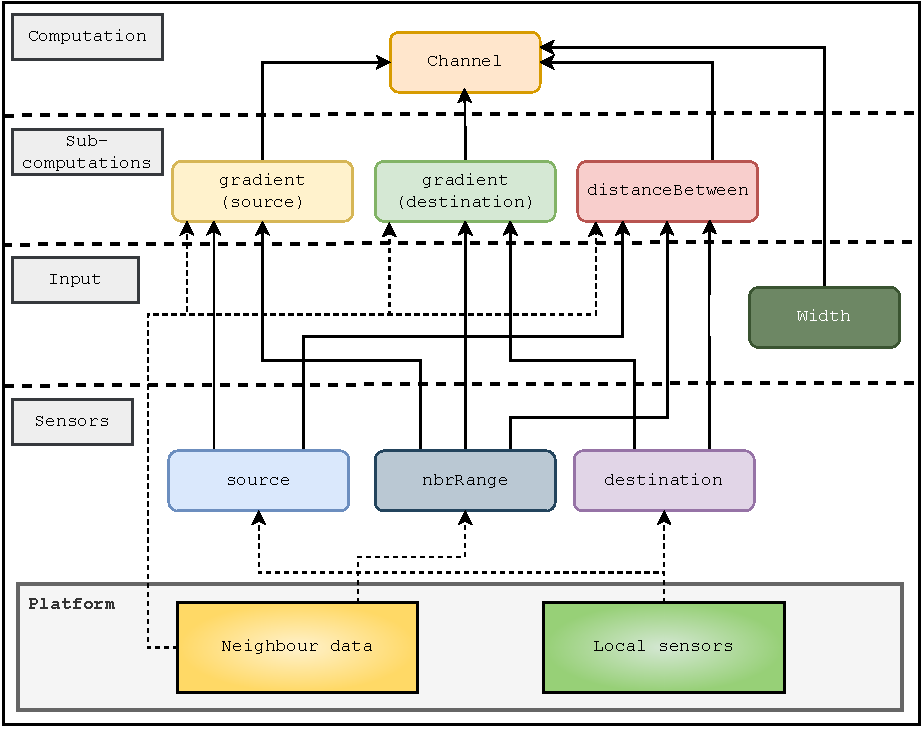
\includegraphics[width=\columnwidth]{papers/acsos2023-frp/imgs/channel-graphical}
    \caption{Node view.}
    \label{acsos2023-frp:fig:channel-graphical}
  \end{subfigure}
  % subfigure
  \begin{subfigure}[b]{\columnwidth}
    \centering%
    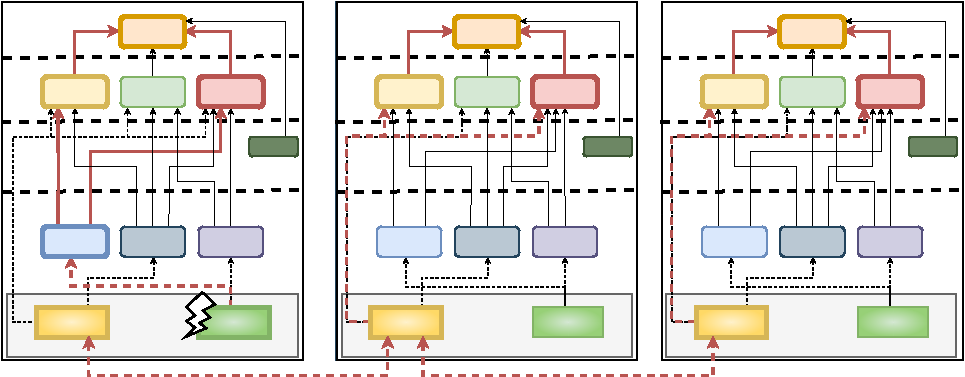
\includegraphics[width=\columnwidth]{papers/acsos2023-frp/imgs/interactions}
    \caption{Distributed view (with neighbour dependencies).}
    \label{acsos2023-frp:fig:interactions}
  \end{subfigure}
  \caption[The reactive dataflow graph corresponding to the channel example.]{
      The reactive dataflow graph corresponding to \Cref{acsos2023-frp:ex:channel}.
      %
      \Cref{acsos2023-frp:fig:channel-graphical} provides the local view of the computation for a single node
      (where the layers denote different semantic kinds of dependencies),
      whereas \Cref{acsos2023-frp:fig:interactions} shows the \emph{distributed} dependency graph.
      %
      The arrows denote dependencies.
      %
      The dashed arrows denote dependencies based on platform-level scheduling and node interaction---e.g.,
      a red block depends on changes corresponding to neighbours' red blocks and communicated via message passing.
  }
  \label{acsos2023-frp:fig:channel:graph}
\end{figure}

\end{example}

\section{Implementation}
\label{acsos2023-frp:sec:impl}

%\meta{
%budget: 1 pages
%}

This section briefly provides the implementation goals (\Cref{acsos2023-frp:sec:impl:goals}), architectural design (\Cref{acsos2023-frp:sec:impl:arch}), and implementation details (\Cref{acsos2023-frp:sec:impl:impl}) of \ac{langname}.
%
Even though a complete description of the implementation is beyond the aims of this paper,
 this section is meant to illustrate that 
 the prototype is technically sound,
 that we followed modern software engineering practices,
 and to provide general guidance for understanding the code organization of the provided artefact (see \Cref{acsos2023-frp:footnote:dsl}).

\subsection{Goals}
\label{acsos2023-frp:sec:impl:goals}

The high-level goal of this work is to provide a programming model
that is expressive enough to allow developers
to declaratively describe \textit{self-organising} collective computations
while decoupling and providing fine-grained control over their scheduling details.
%
This vision can be summarized with the term \textit{functional reactive self-organization}.
%
Considering the system model introduced in \Cref{acsos2023-frp:sec:sys-model},
 there are three main objectives to be pursued in order to accomplish the goal:
%
\begin{itemize}
    \item \emph{Re-compute only upon \emph{relevant} changes in the context}: computations should occur reactively only when relevant changes are observed from the environment (i.e., sensing and neighbour data). %, in order to avoid wasteful resources usage;
    \item \emph{Avoid re-evaluation of unaffected sub-computations}: if a portion of the computation depends on data that did not change, it should not be re-evaluated.
    \item \emph{Interact only upon relevant changes}: each device should avoid broadcasting an export that did not change since the last one, with the direct consequence that no further message exchange should be required if a computation reaches a stable configuration.
\end{itemize}

\subsection{Architecture}
\label{acsos2023-frp:sec:impl:arch}

The architecture of the prototype is shown in \Cref{acsos2023-frp:fig:arch}.
%
The design is organised into three packages:
    \texttt{core},
        which includes basic type definitions
        (\texttt{Core}) as well as the components for the \ac{dsl}
        (\texttt{Language} for primitives and \texttt{RichLanguage} for other built-ins)
        and its ``virtual machine'' (\texttt{Semantics}),
        overall captured by an \texttt{Incarnation};
    \texttt{frp},
        which provides an interface to the \ac{frp} engine (\texttt{FrpEngine}),
        possibly also decoupling from the specific \ac{frp} library adopted,
        as well as extensions (\texttt{FrpExtensions}) useful for the definition of \ac{langname} constructs;
    and \texttt{simulation},
        which provides basic simulation support
        (for more advanced support, we also integrated \ac{langname} into Alchemist~\cite{PianiniJOS2013}---see \Cref{acsos2023-frp:sec:eval}).

\begin{figure}
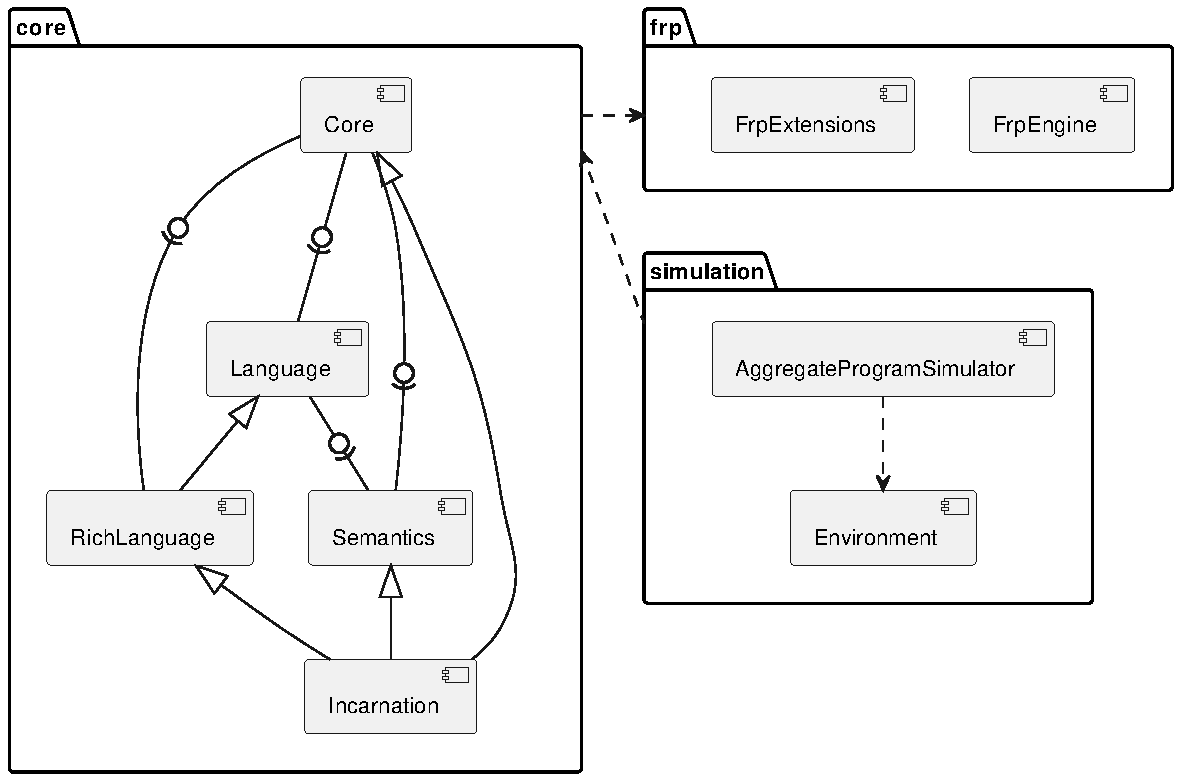
\includegraphics[width=\columnwidth]{papers/acsos2023-frp/imgs/architecture.pdf}
\caption{Architecture of \ac{langname}.}
\label{acsos2023-frp:fig:arch}
\end{figure}


\subsection{Implementation details}
\label{acsos2023-frp:sec:impl:impl}

\ac{langname} has been implemented in Scala,
 using Sodium as \ac{frp} library~\cite{blackheath2016frp-sodium}.
%
Scala is well-known for its suitability
 as a host for embedded \acp{dsl}~\cite{DBLP:conf/icfem/ArthoHKY15},
and for aggregate computing embeddings as well~\cite{DBLP:journals/lmcs/AudritoCDV23}. %DBLP:journals/infsof/KosarBM16,
%
The design of the \ac{langname} \ac{dsl}
 is detailed in \Cref{acsos2023-frp:fig:dsl-design}.

Following the system/execution model described in \Cref{acsos2023-frp:sec:sys-model},
  we model the input and output 
  of a (sub-)program 
  through an interface \texttt{Context},
  providing access to local sensor data and neighbour data;
  and an interface \texttt{Export},
  capturing outputs and data that must be shared with neighbours.
%
In particular, an \texttt{Export} 
 is modelled as a \emph{tree}
 where each node is a \texttt{Slot}
(corresponding to a particular language construct)
with an associated value,
 and can be located through a \emph{path} of slots---e.g.,
\texttt{S1/S2/S3} identifies a node in the export tree,
where \texttt{S1} depends on \texttt{S2} which depends in turn on \texttt{S3}
(so, a change in the output \texttt{S3} will cause the expression corresponding to \texttt{S2} to re-evaluate, and possibly \texttt{S1} in turn).

\texttt{Flow} is the type 
 of a reactive \mbox{(sub-)computation},
 which takes a \texttt{Context} (providing its inputs),
 a \texttt{Seq[Slot]} as path (indicating its position in the export tree),
 and returns \texttt{Cell} (i.e. a time-varying value---cf. \Cref{acsos2023-frp:sec:background:frp}) of \texttt{Export}.
%
Each \texttt{Language} construct
 returns a \texttt{Flow}:
 therefore, the constructs do \emph{not} immediately run upon evaluation,
 but rather an executable, reactive object
 denoting a computation graph
 whose nodes will execute as a response to change (cf. \Cref{acsos2023-frp:fig:channel:graph}).
%
Access to neighbour-related data is mediated by a \texttt{NeighborField} abstraction,
 which is the same provided by constructs
 supporting interaction with neighbours, i.e., \texttt{nbr} and \texttt{nbrSensor}
(cf. \Cref{acsos2023-frp:programming-constructs}).

\begin{figure}
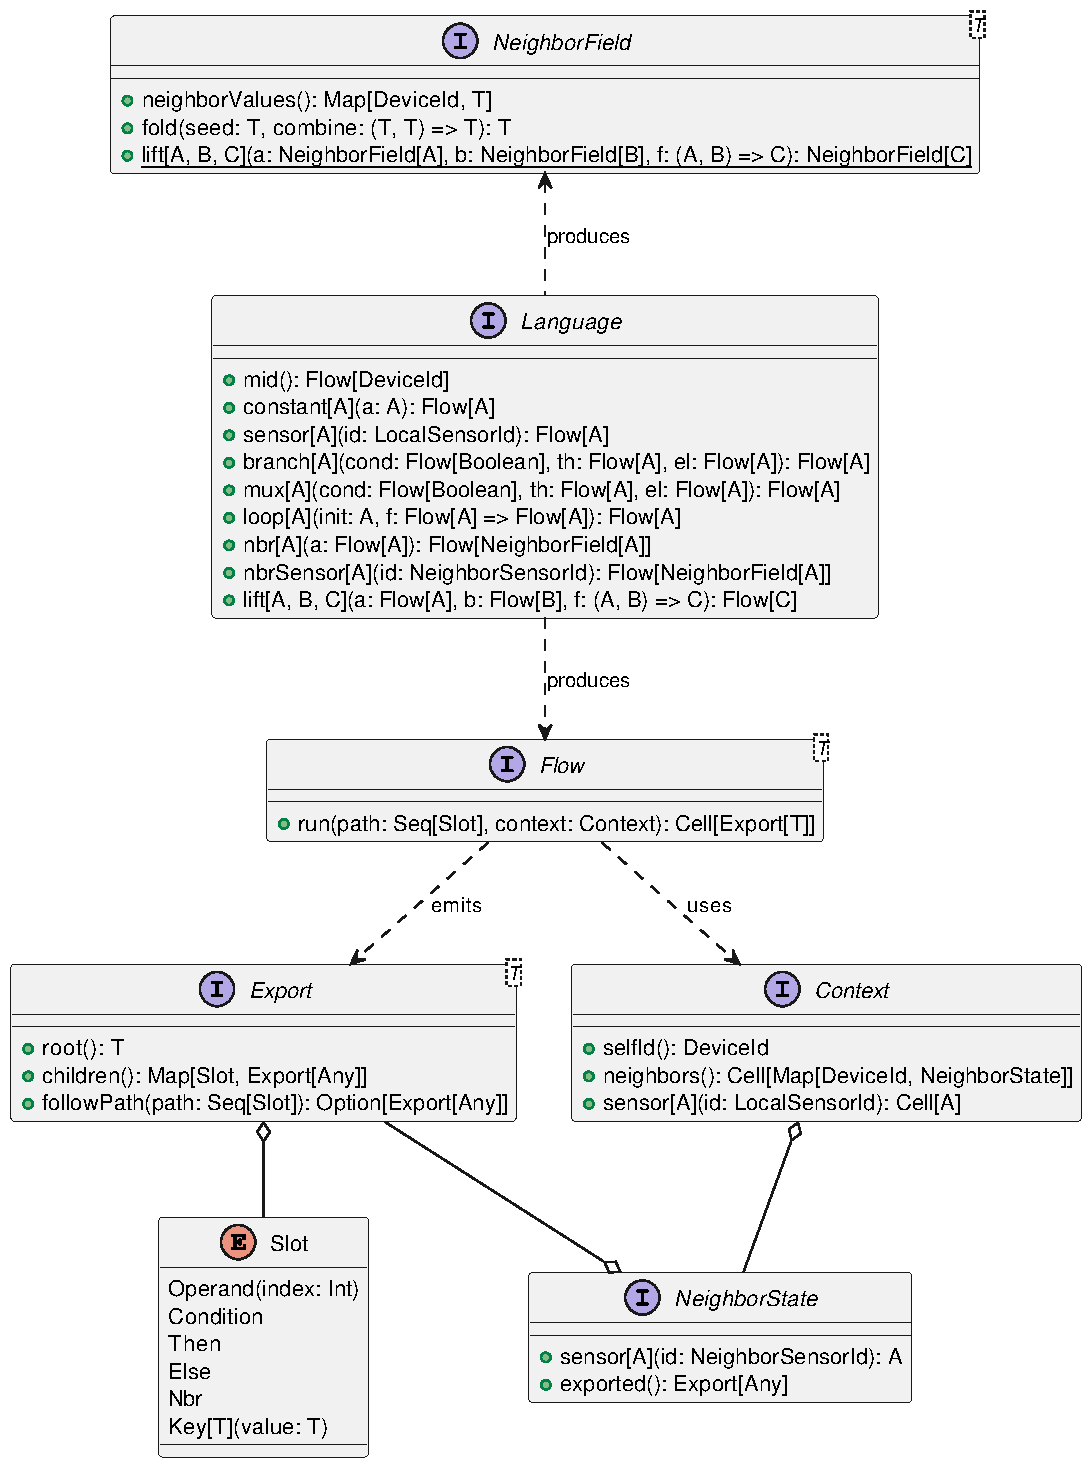
\includegraphics[width=\columnwidth]{papers/acsos2023-frp/imgs/specification.pdf}
\caption{Design of \ac{langname} \ac{dsl}.}
\label{acsos2023-frp:fig:dsl-design}
\end{figure}

\section{Evaluation}
\label{acsos2023-frp:sec:eval}

%\meta{
%budget: 2,5 pages
%
%SECTION IDEA: compare reactive impl of gradient from standard proactive impl of gradient and show that we are more efficient (the reactive version runs less rounds, i.e., no need for computing when there is no change)
%}

To evaluate the proposed approach, 
 we prepared several publicly available and reproducible simulations
(see \Cref{acsos2023-frp:footnote:eval}) using the \emph{Alchemist} simulator for large-scale pervasive systems\footnote{\url{https://alchemistsimulator.github.io/}}~\cite{PianiniJOS2013}.
%
In particular, 
 we released \ac{langname}\footnote{\url{https://central.sonatype.com/artifact/io.github.cric96/distributed-frp_3/0.1.3}} and integrated it into Alchemist.
%
The choice of Alchemist allowed us to leverage the already integrated \emph{\scafi{}} aggregate programming language~\cite{DBLP:journals/softx/CasadeiVAP22}
as a reference for round-based computations (cf. \Cref{acsos2023-frp:sec:background:selforg}).

\subsection{Goals}\label{acsos2023-frp:eval:goals}
%
The simulations are designed to evaluate the following:
%
\begin{enumerate}
\item[G.1)] \emph{Correctness}: the reactive and round-based versions of the same algorithm should ultimately produce the same correct collective results.
\item[G.2)] \emph{Efficiency}: The efficiency is measured in terms of:
\begin{enumerate}
  \item \emph{messages}: the number of messages exchanged between devices;
  \item \emph{time}: the time required to reach a stable output;
  \item \emph{computation}: the number of sub-computation steps performed by each device.
\end{enumerate}
In particular, we expect the reactive version of the algorithm to be \emph{more efficient} than the round-based one.
\item[G.3)] \emph{Reactivity}: the programs should react to various sources of change
 (e.g., network topology, sensor data, dependent computations---cf. \Cref{acsos2023-frp:sec:sys-model}),
  avoiding re-evaluations when inputs do not change.
%(e.g., change in the network topology, change in source set, etc.).
\end{enumerate}
%\meta{TODO}

\subsection{Experimental Setup}
\begin{figure}
  \centering
    \begin{subfigure}[b]{0.49\linewidth}
        \centering
        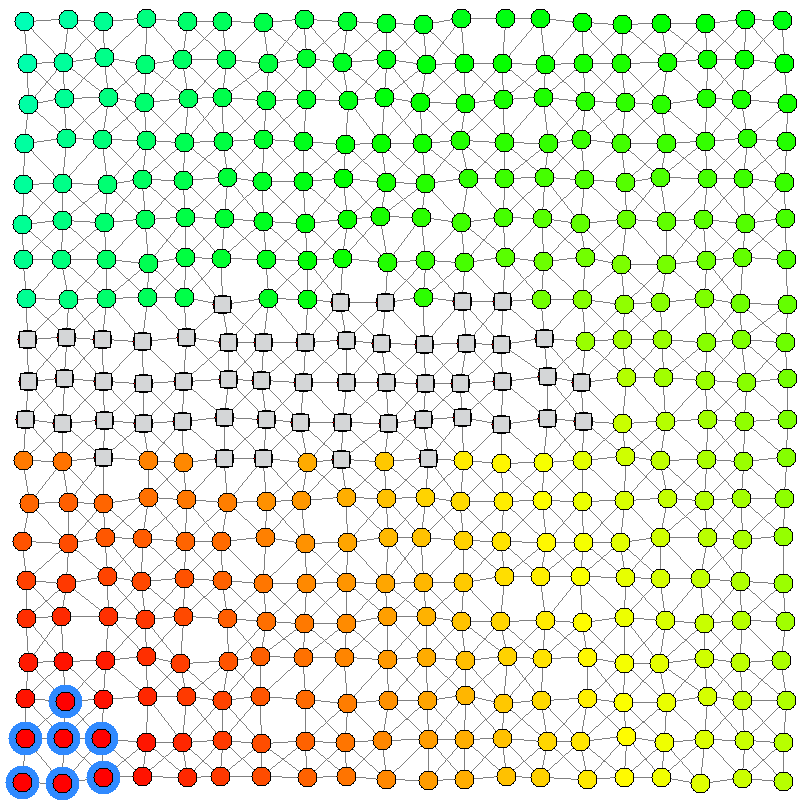
\includegraphics[width=\textwidth]{papers/acsos2023-frp/imgs/gradient.png}
       \caption{Scenario G: gradient.}
        \label{acsos2023-frp:fig:scenario-g}
    \end{subfigure}
    \begin{subfigure}[b]{0.49\linewidth}
        \centering
        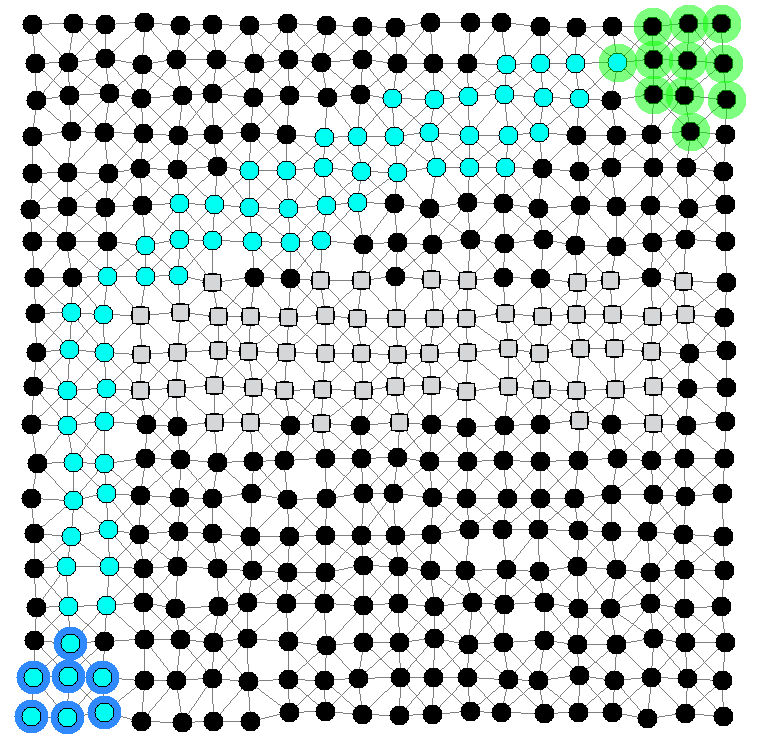
\includegraphics[width=\textwidth]{papers/acsos2023-frp/imgs/channel.png}
        \caption{Scenario C: channel.}
        \label{acsos2023-frp:fig:scenario-c}
    \end{subfigure}
    \caption[Evaluation scenarios implemented with \ac{langname}]{
      Evaluation scenarios.
      The output of the program being evaluated is depicted in the inner circle. 
      On the left, the hue varies depending on the gradient output, with redder colours indicating lower values. 
      On the right, the channel between the source nodes (blue shadow) and destination (green shadow) is indicated in cyan.
%      The outer circle represents sensor information, with yellow nodes indicating the presence of a source and green nodes indicating the presence of a destination. 
      The grey nodes denote obstacles. % that the program must navigate around to reach the destination.
    }
    \label{acsos2023-frp:fig:scenario-screenshots}
\end{figure}

\subsubsection{Common setup and parameters}
%
The simulated system consists of 400 devices 
 placed on a $100 m \times 100 m $ square and forming a slightly irregular grid
(nodes' positions are generated for a regular grid and then randomly deviated).
%
Each node has a mean distance to its neighbours of 5 meters
 and a communication radius of 7.5 meters. 
%
Messages sent by the nodes may be subject to a communication delay
 regulated by the parameter $\tau$, which describes an exponential probabilistic function.
%
Each simulation is characterized by the mode of execution of the aggregate program,
 which can be 
 (i) \emph{purely reactive}, 
 (ii) \emph{reactive with throttling}, or 
 (iii) \emph{round-based}. 
%
The pure reactive policy is evaluated for every new message received from any neighbour.
%
This policy is expected to converge quickly
at the price of a significant overhead in the number of exchanged messages.
% 
The ``reactive with throttling'' policy
 is %a reactive policy
 parametrized on the throttling frequency $\gamma$
(i.e.,  the inverse of the period in which all events received in this interval are accumulated before emission).
%
Compared to the purely reactive policy,
  throttling is expected to reduce message overhead at the expense of convergence time. 
%
Finally, the round-based policy is driven by a $\gamma$ parameter
 describing how often each device will wake up and compute the round.

\subsubsection{Scenarios}

In the above setup, the two programs introduced in \Cref{acsos2023-frp:sec:contrib},
 i.e., the self-healing gradient (\emph{scenario G}---cf. \Cref{acsos2023-frp:fig:scenario-g}) and channel (\emph{scenario C}---cf.~\Cref{acsos2023-frp:fig:scenario-c}),
 are executed for 300 simulated time units. 
%
The former represents a minimally complex self-organising behaviour, enabling evaluation of basic dynamics, 
 whereas the latter is representative of larger behaviours that can be defined as compositions of simpler ones, hence 
 providing insights about what could happen when multiple reactive computations are combined.

For \emph{scenario G},
 a group of nodes (i.e., a $20m \times 20m$ area at the bottom left) is marked as gradient source.
%
Also, a set of nodes marked as obstacles is positioned at the centre in a $8m \times 2m$ area.
%
To verify that the gradient can adapt to changes and assess the effects of continuous and frequent changes in the system,
at simulated time $t=150$ a cluster of nodes migrates from the lower left-hand side to the lower right-hand side of the area.

For \emph{scenario C},
 a set of nodes denoting the channel's destination are placed in the upper right in a $20m \times 20m$ area.
 Here, to verify reactivity to change, 
 we switch the set of destination nodes at $t=200$ 
 from the upper-right corner to the upper-left corner. 
This injected change allows us to observe both
 the channel computation's reactivity and the sub-computations' evaluation.
 In fact, by only modifying the destination area, the gradient starting from the source (which is a sub-computation of the channel computation) should not be re-evaluated (as it would not change its collective output).

\subsubsection{Metrics}

The metrics extracted for this study are:
\begin{itemize}
  \item \emph{Total cumulative number of messages exchanged (up to time $T$)}  -- \texttt{\#messages}: 
 this is used to evaluate the communication overhead/efficiency (cf.\ goal G.2)
 and to inspect the communication dynamics of the reactive solution.
%  one of the key points in our new computation model is to create more efficient programs in terms of messages exchanged between the nodes in the system (goal 2.B). For a certain time $t$, this value will be calculated as: 
  It is computed as the sum of the number of messages sent by each node up to time $T$.
  %\begin{equation}
  %\text{\#messages}(T) = \sum_{i=1}^{n}\int_{t=0}^{T}messages_i(t)dt
  %  \end{equation}
  %where $messages_i(t)$ is the number of messages sent by node $i$ at time $t$.
%  This metric will also allow us to observe the responsiveness of the system, as we expect that, in case of variations in sensors, the nodes start to send new messages.
    
  \item \emph{Average output value of the system} -- \texttt{output (mean)}: for each time instant $t$, we extract the average value of the computational field produced by the system.
  %\begin{equation}
  %\text{output}(t) = \frac{1}{n}\sum_{i=1}^{n} x_i(t)
  %\end{equation}
  %where $x_i(t)$ is the output produced by node $i$ at time $t$.
  This value will allow us to assess both correctness (cf.\ goal G.1)
  and time efficiency (when the programs converge to a certain stable value---cf.\ goal G.2).
  %
  Also, this indicates the responsiveness of the system, as the output should vary with the introduction of changes in the system.
  
  \item \emph{Total number of executions for program sub-computations} -- \texttt{\#evaluations}:
  this value was extracted in the channel program only (since it comprises multiple subprograms).
  For each sub-program, we calculated the number of times it has been evaluated up to time $T$ as the sum of the number of evaluations of each node.

  %\begin{equation}
  %  \text{\#evaluations(T,L)} = \sum_{i=1}^{n}\int_{t=0}^{T}evaluations_i(t,L)dt
  %\end{equation}
  %where $evaluations_i(t,L)$ is the number of times the subprogram $L$ had been evaluated by node $i$ at time $t$.
  This metric is useful for assessing goals G.2c and G.3. %, as we would like to see that when a certain subprogram does not need to be evaluated, this actually happens:
  
\end{itemize}

\subsubsection{Baselines}

To establish baselines, 
 we implemented round-based solution programs for the self-healing gradient (scenario G) and channel (scenario C) in \scafi{}---see~\cite{DBLP:journals/softx/CasadeiVAP22}. 
% The syntax of the two domain-specific languages is similar, as evidenced by the gradient expressed in this framework:
%\begin{lstlisting}
%def gradient(source: Boolean): Double = {
%  rep(Double.PositiveInfinity) { distance =>
%    mux(source) { 0.0 } {
%      minHoodPlus(nbr(distance) + nbrRange())
%    }
%  }
%} 
%\end{lstlisting}
%Where \lstinline|rep| is the counterpart of \lstinline|loop| 
% of the proposed DSL, and \lstinline|minHoodPlus| produces the minimum value of the neighbourhood without the value of the node itself.
%
The execution for the round-based solution is configured 
 with an evaluation frequency of 1Hz: any device will evaluate the entire ScaFi program every second
 and then broadcast the resulting export to its neighbourhood (even if it did not change from the previous execution).

\subsection{Results and Discussion}\label{acsos2023-frp:eval:results}
%
In this section, we will present the results obtained from the simulations, 
 highlighting how the proposed model satisfies the goals elicited in \Cref{acsos2023-frp:eval:goals}.
%
We run a total of 768 simulations
by running 64 randomized instances
(varying the random seed and the position of the nodes in the environment)
for each one of the $12$ \emph{simulation configurations} obtained by a different combination of
\textit{(i)} execution mode,
\textit{(ii)} throttling period, and
\textit{(iii)} scenario program.
%
Our results are presented in \Cref{acsos2023-frp:fig:rel-values} and \Cref{acsos2023-frp:fig:subprogram-eval}.
%\Cref{acsos2023-frp:fig:channel-messages-rel} and \Cref{acsos2023-frp:fig:gradient-messages-rel} for the gradient and the channel, respectively, averaging the data extracted.
%%% GOAL 1 

\subsubsection{Correctness (goal G.1)} Consider \Cref{acsos2023-frp:fig:channel-output-rel} and \Cref{acsos2023-frp:fig:gradient-output-rel}:
 we observe that in all cases,
especially in the reactive and throttling executions,
 the program output converges to the same collective result.
%
Pure reactive policies have less noise (as variations are reduced)
 but tend to converge to the same result on average.

%%% GOAL 2

\subsubsection{Efficiency (goal G.2)} 
%
From~\Cref{acsos2023-frp:fig:rel-values},
we can see how the reactive computation is more efficient than the round-based one
(cf.\ goal G.2)
in the sense of communication/computation efficiency
(\Cref{acsos2023-frp:fig:channel-messages-rel,acsos2023-frp:fig:gradient-messages-rel})
and time efficiency (\Cref{acsos2023-frp:fig:gradient-output-rel,acsos2023-frp:fig:gradient-output-rel}).
%
Moreover, as expected, throttling can further improve the efficiency of the reactive solution.


Indeed, starting with the messages metric, we observe that 
 the number of messages exchanged in pure reactive policies to reach a stable output is greater than the throttled counterpart.
%  
This result is expected:
 in the purely reactive model
 each message different from a previous one
 causes a program re-evaluation and subsequent message sending.
%
Analysing the policies with throttling, 
 we notice that the higher the throttling period, 
 the lower the number of messages sent, 
 and in particular, the 
 more the policy tends towards the round-based one.
% 
In the gradient scenario, for instance, 
 the throttle mode achieves convergence 
 by sending six times fewer messages than the round-based one.
%
Despite consuming more, 
 purely reactive policies are still more efficient than round-based ones,
sending approximately 40\% less messages.
%
However, it is also noteworthy that, 
 in the case of continuous variations, 
 such as the migration of nodes in the gradient scenario,
the number of messages grows linearly in both reactive and round-based modes.
%
%This is inevitable since any environmental changes will cause a re-evaluation with subsequent sending of messages.
%
Efficiency could be improved by approximating the output value
not to send every message for every update,
i.e., to regulate reactivity according to some threshold for ``significant change''.

Moving on to converge time, 
 we immediately note that reactive policies are the most efficient
 because they expand changes throughout the system as soon as they occur, 
 avoiding delays due to waiting for a new evaluation round.
%
However, in the case of frequent environmental change, 
 one may have a higher message consumption than round-based policies, 
 leading to higher energy consumption.

Observing throttling policies, 
 we note that the higher the throttling period, 
 the higher the convergence time, 
 as the system will take longer to react to changes.
%
In the worst case 
 (i.e., when the throttling period is equal to the evaluation time of round-based policy), 
 the convergence time is approximately the same.
%
However,
convergence time shortens with the decrease in the throttling period,
getting performance close to the purely reactive policy
but with fewer messages exchanged.
%
Thus, 
\emph{the proposed model balances communication cost
    (the number of messages exchanged)
    and performance
    (time required to converge to the expected output),
    depending on the application's needs}.
%
Moreover,
the relationship between the throttling period and
the number of messages sent is not linear
(unlike the convergence time).
%
In fact,
halving the period (0.5 seconds instead of 1 second)
also halves the convergence time,
yet
the number of messages exchanged is approximately the same.

%%% GOAL 3
Concerning reactivity (goal G.3), 
 we notice how the reactive solutions effectively ``follow'' environmental changes.
%
This can be observed from 
  \Cref{acsos2023-frp:fig:channel-messages-rel} and \Cref{acsos2023-frp:fig:gradient-messages-rel}:
  when there is no change to react to, 
 no program evaluation is performed, 
 resulting in no new messages being sent
 (cf.\ the intervals where the message count does not increase).
%
Moreover, as the environmental conditions vary, 
 the program is re-evaluated, as observed at the moment of variation
(at $t=150$ in the case of the gradient and at $t=200$ in the case of the channel).
 
Finally, we show how the model promotes \emph{fine-grained reactivity}.
%
\Cref{acsos2023-frp:fig:subprogram-eval} shows how
 \ac{langname} enables a program to re-compute required sub-computations \emph{only}.
%
Indeed, at $t=200$, only the channel's target changes,
and thus the source gradient is not re-computed
(it would be pointless since its inputs did not change).
%
Also, this execution occurs only where needed, 
 resulting in a ``wave'' of re-computations from the source to the destination
(cf.\ the larger red circles in \Cref{acsos2023-frp:fig:subprogram-eval}).

\begin{figure}
  %% Subfigures for the channel-messages-rel, channel-output-rel, gradient-messages-rel and gradient-output-rel
  \centering
  \begin{subfigure}[b]{\linewidth}
      \centering
      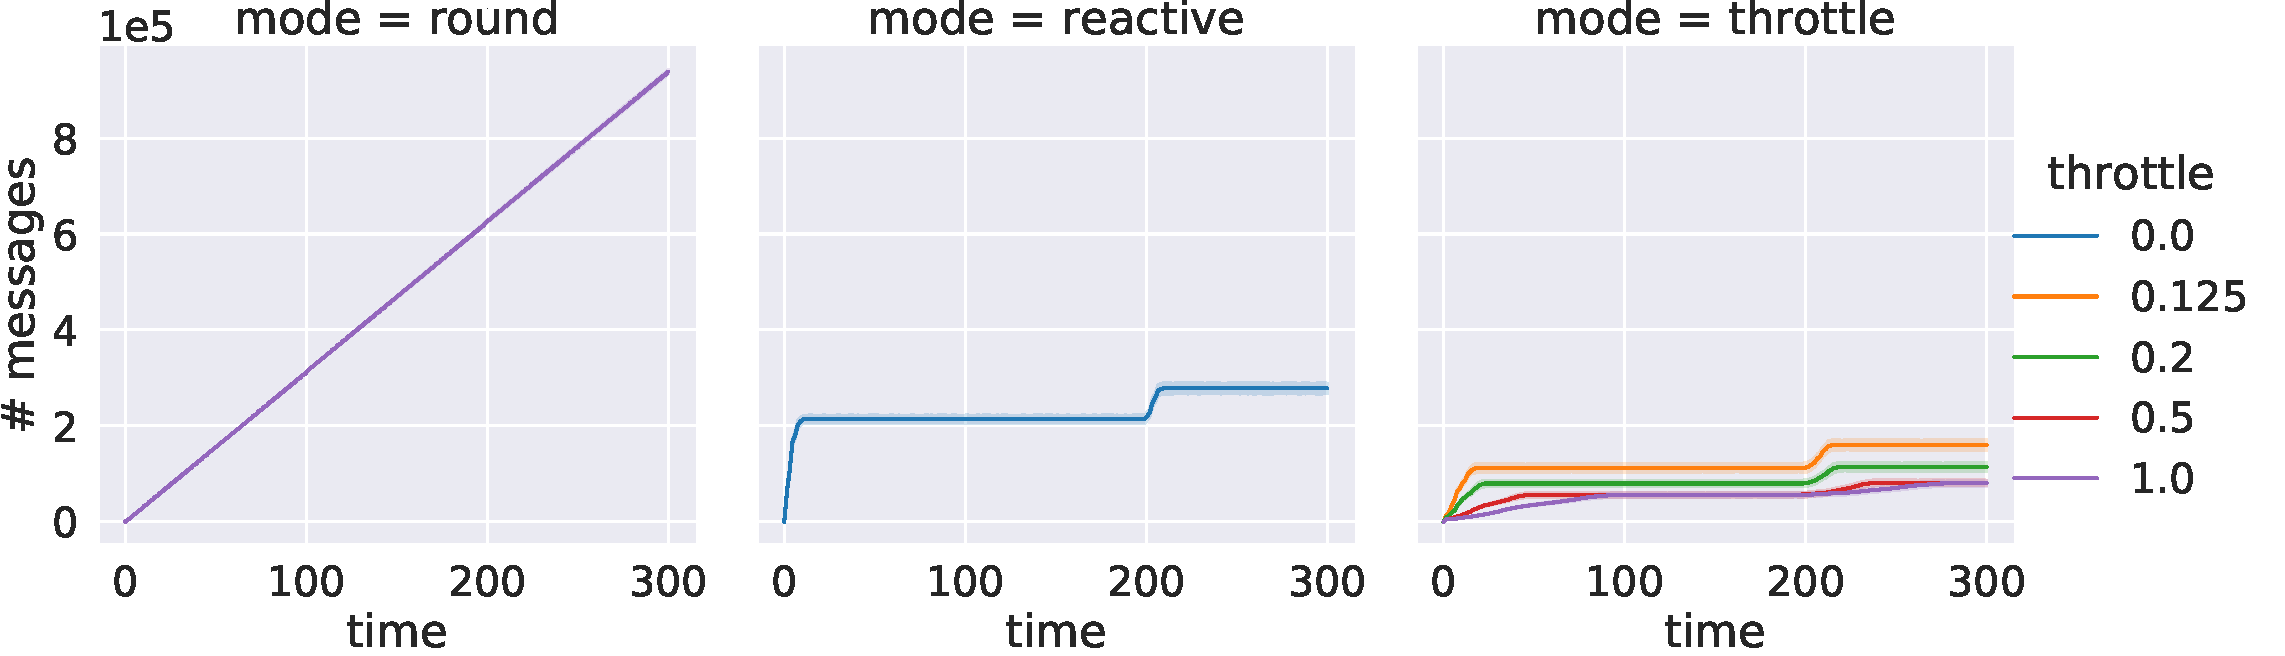
\includegraphics[width=\textwidth]{papers/acsos2023-frp/imgs/channel-messages-rel}
      \caption{Channel: messages.}
      \label{acsos2023-frp:fig:channel-messages-rel}
  \end{subfigure}
  \begin{subfigure}[b]{\linewidth}
      \centering
      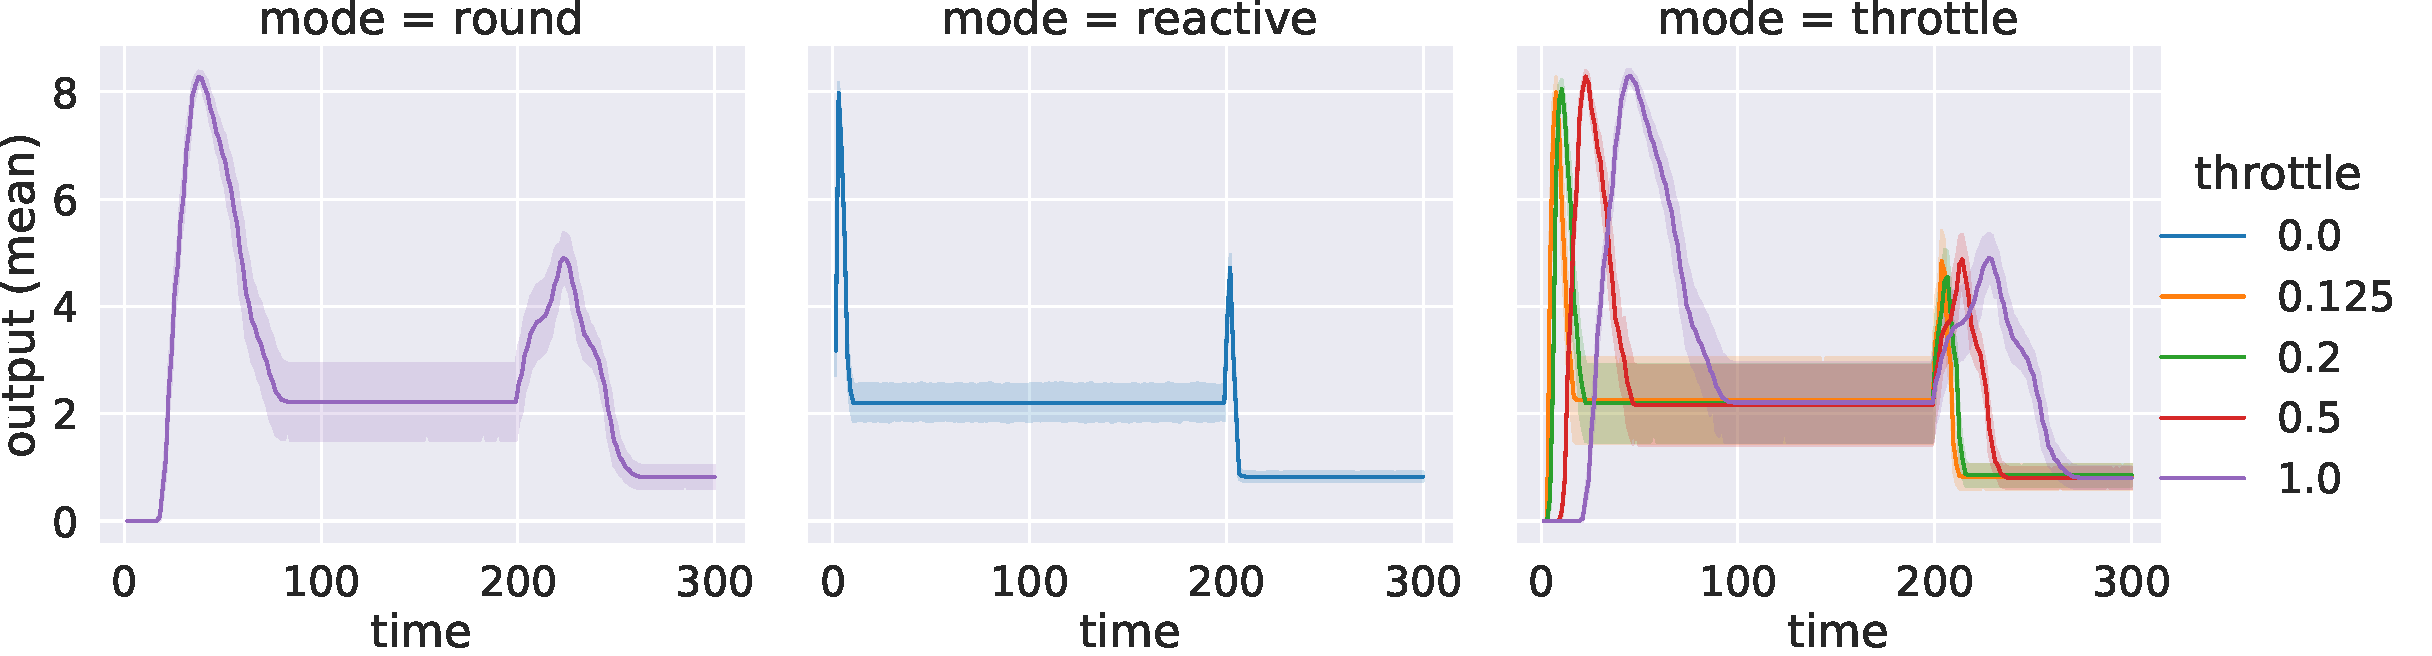
\includegraphics[width=\textwidth]{papers/acsos2023-frp/imgs/channel-output-rel}
      \caption{Channel: output.}
      \label{acsos2023-frp:fig:channel-output-rel}
  \end{subfigure}
  \begin{subfigure}[b]{\linewidth}
      \centering
      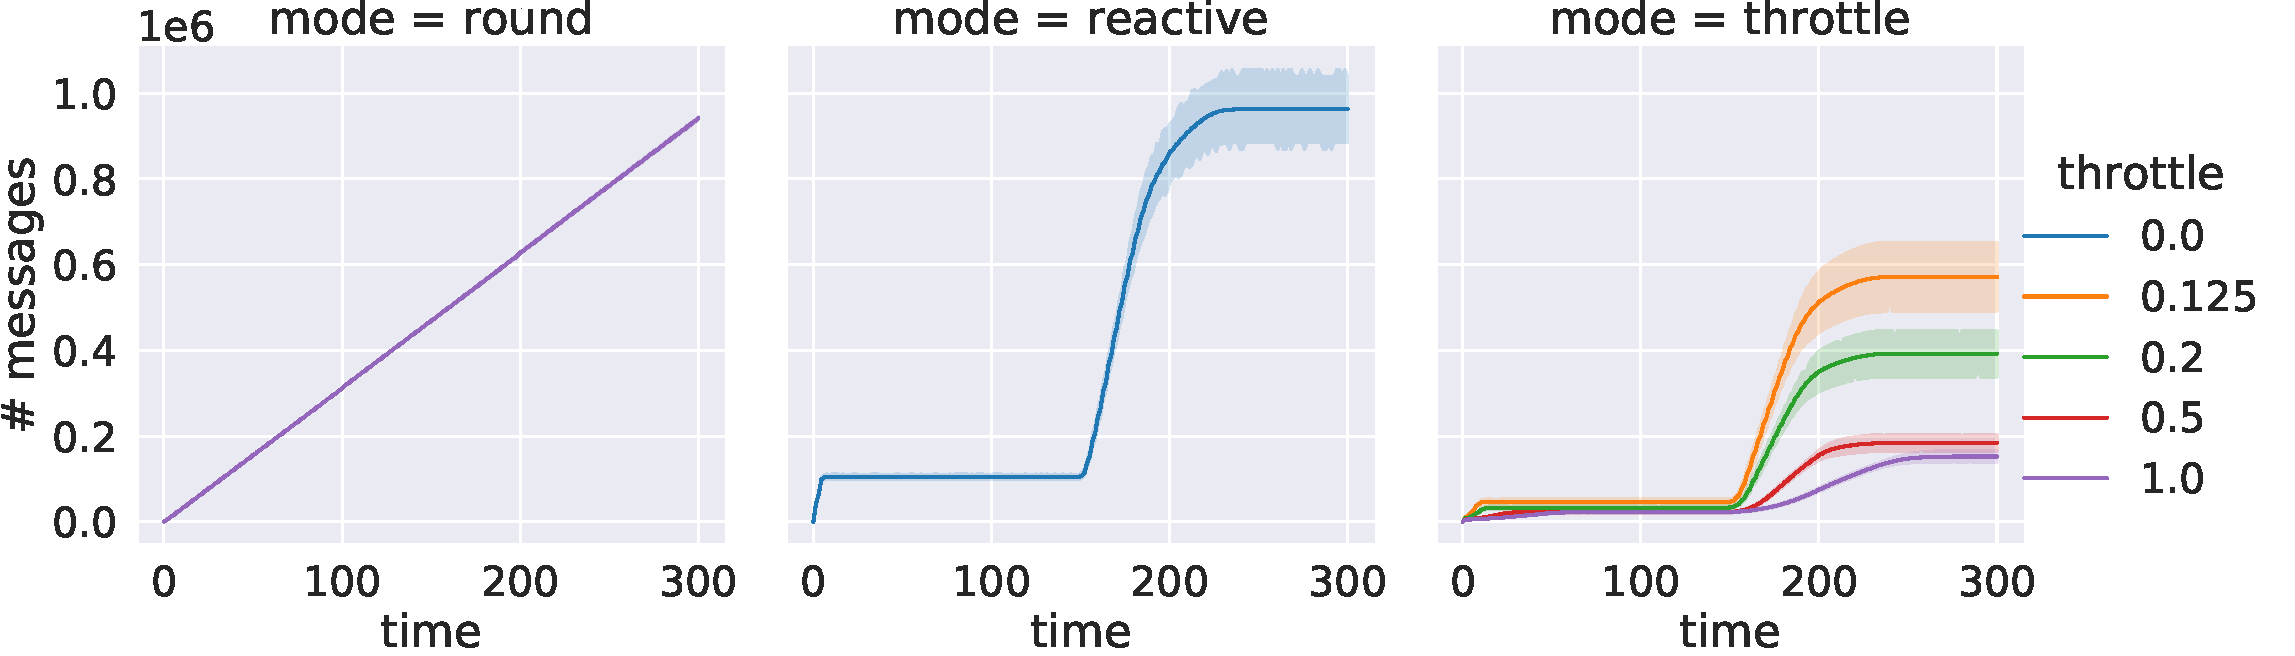
\includegraphics[width=\textwidth]{papers/acsos2023-frp/imgs/gradient-messages-rel}
      \caption{Gradient: messages.}
      \label{acsos2023-frp:fig:gradient-messages-rel}
  \end{subfigure}
  \begin{subfigure}[b]{\linewidth}
      \centering
      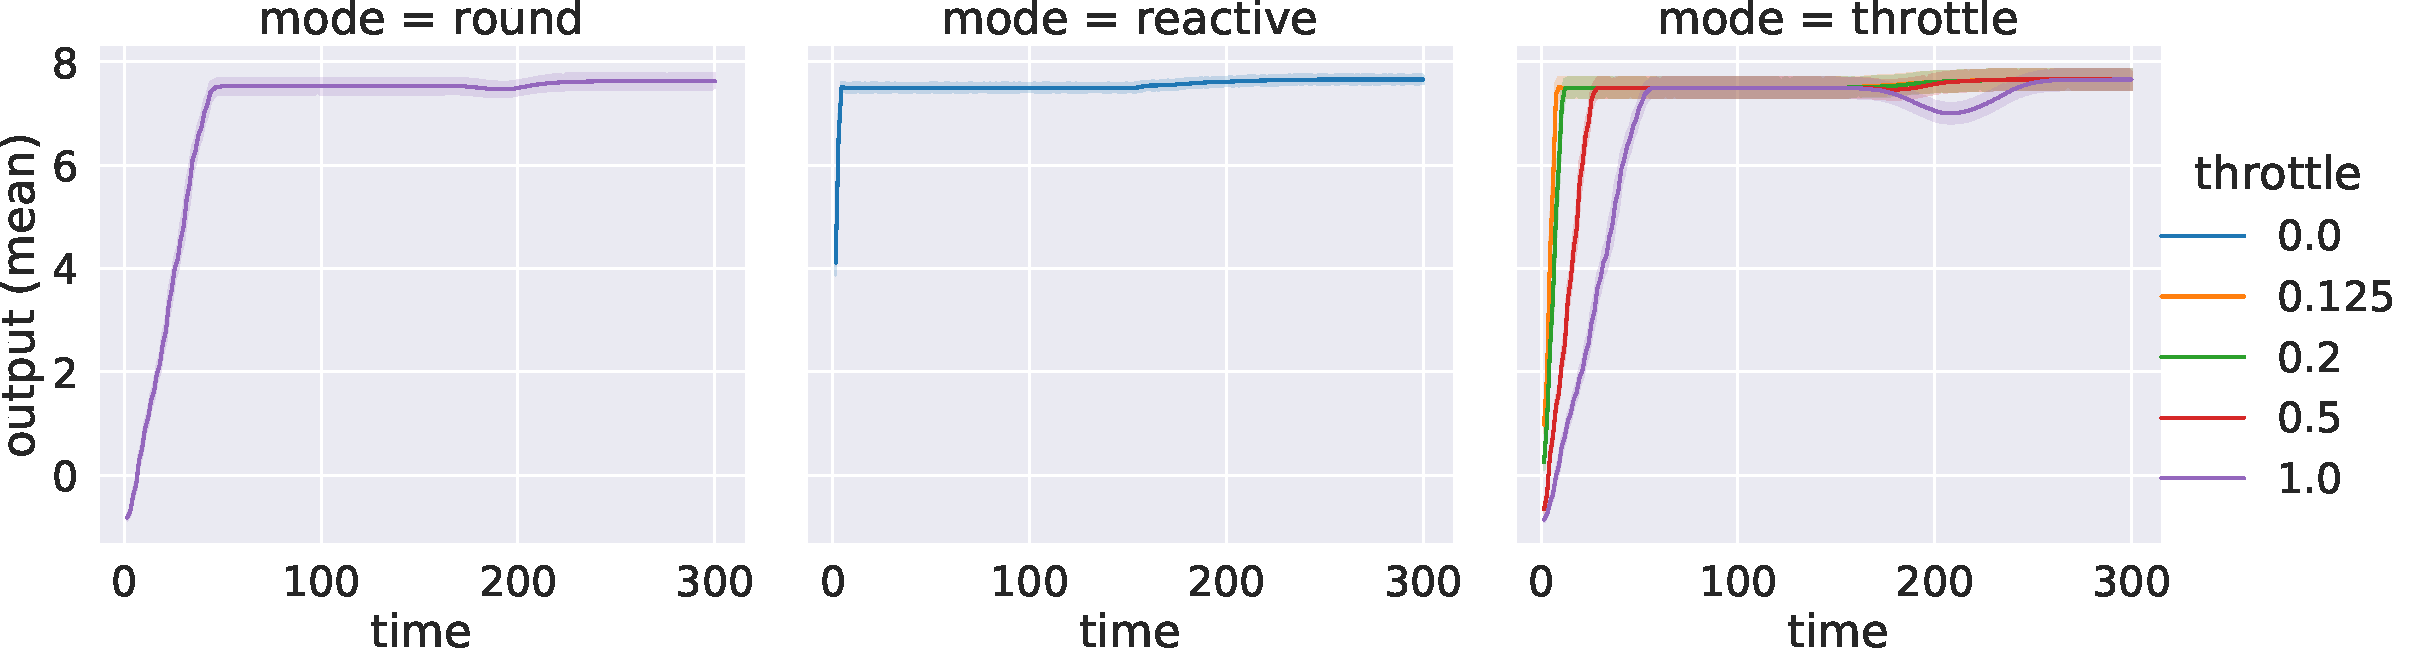
\includegraphics[width=\textwidth]{papers/acsos2023-frp/imgs/gradient-output-rel}
      \caption{Gradient: output.}
      \label{acsos2023-frp:fig:gradient-output-rel}
  \end{subfigure}
  \caption[Simulation results of \ac{langname} simulations]{
    Simulation data.
    %
    The output value (lines 2 and 4)
    from the round-based solution (left column) 
    can be used as a reference to verify the correctness of the computation and the performance
    of the reactive solutions (middle and right columns).
    %
    The number of messages (lines 1 and 3), instead,
    provides an indication of the communication overhead.
    We observe that purely reactive (middle column) and throttled (right column) policies
    convergence to correct values faster than the round-based version;
    also, their communication overhead does not grow with time, but depends on changes.
  }
  \label{acsos2023-frp:fig:rel-values}
\end{figure}
\begin{figure*}
  %% Subfigure for init, expansion, revaluation and finish
  \centering
  \begin{subfigure}[b]{0.24\linewidth}
      \centering
      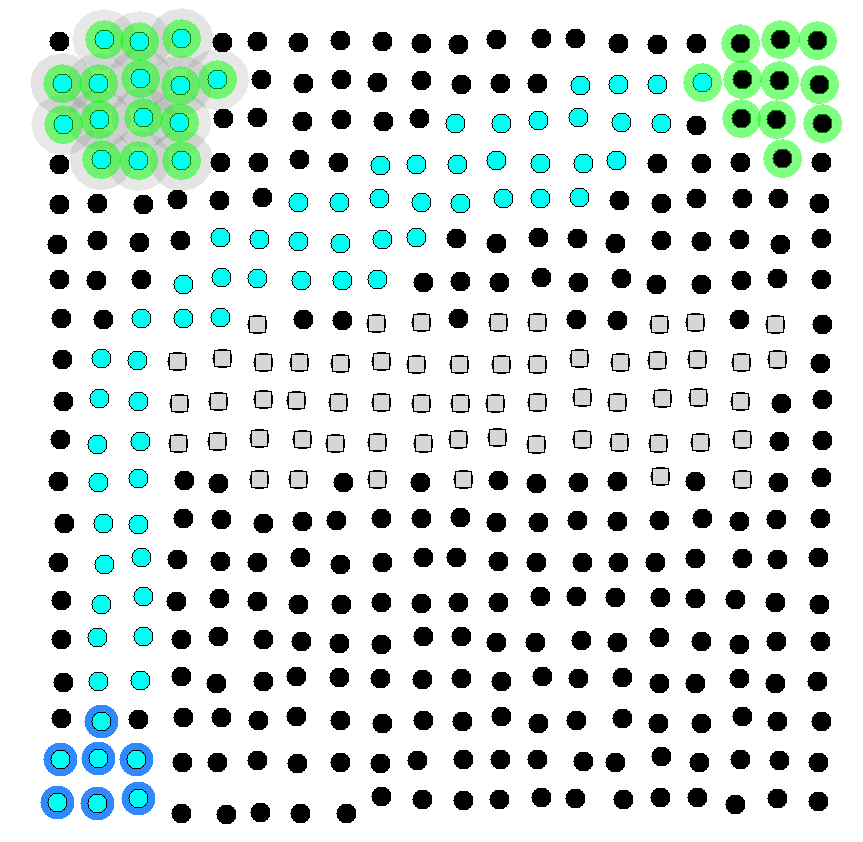
\includegraphics[width=\textwidth]{papers/acsos2023-frp/imgs/channel201.0.png}
      \caption{}
      \label{acsos2023-frp:fig:init}
  \end{subfigure}\hfill
  \begin{subfigure}[b]{0.24\linewidth}
      \centering
      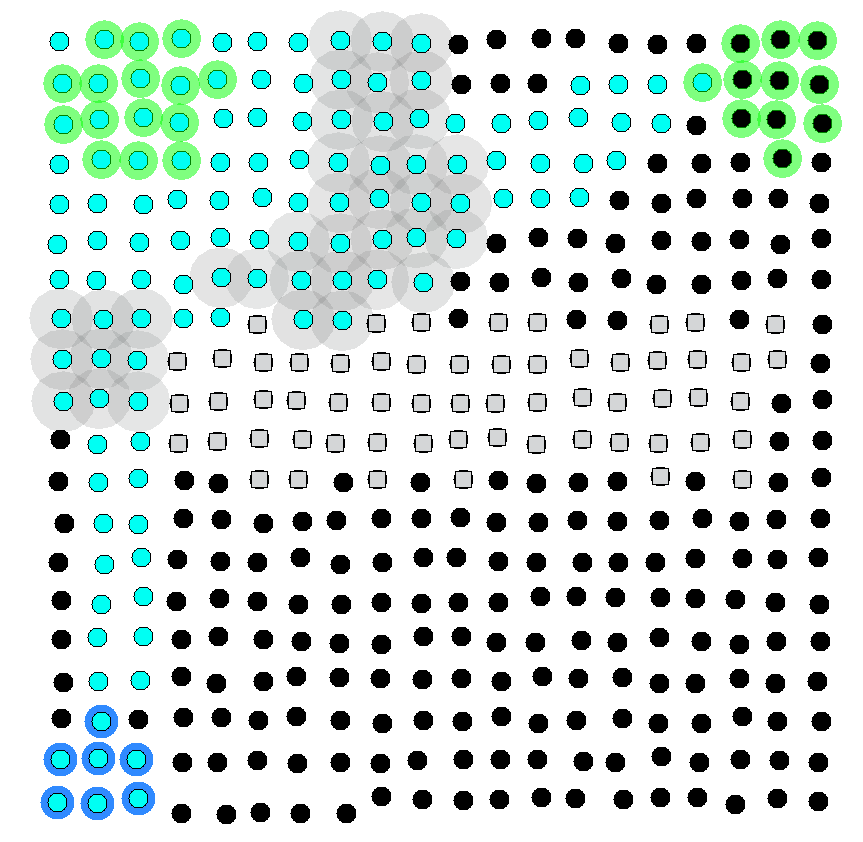
\includegraphics[width=\textwidth]{papers/acsos2023-frp/imgs/channel210.0.png}
      \caption{}
      \label{acsos2023-frp:fig:expansion}
  \end{subfigure}\hfill
  \begin{subfigure}[b]{0.24\linewidth}
      \centering
      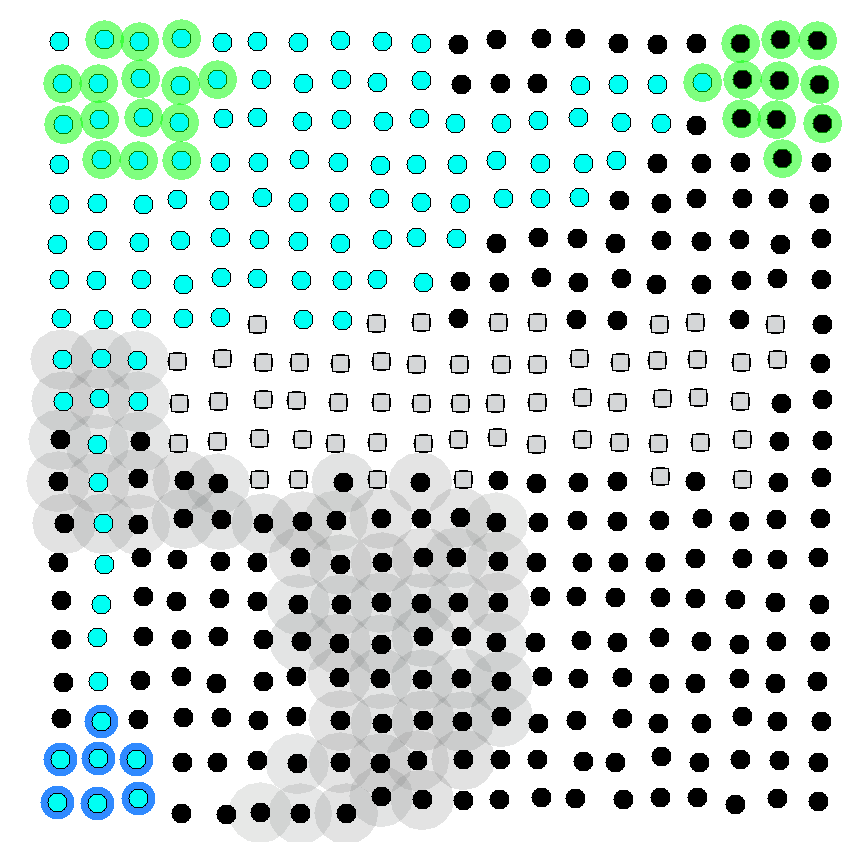
\includegraphics[width=\textwidth]{papers/acsos2023-frp/imgs/channel240.0.png}
      \caption{}
      \label{acsos2023-frp:fig:revaluation}
  \end{subfigure}\hfill
  \begin{subfigure}[b]{0.24\linewidth}
      \centering
      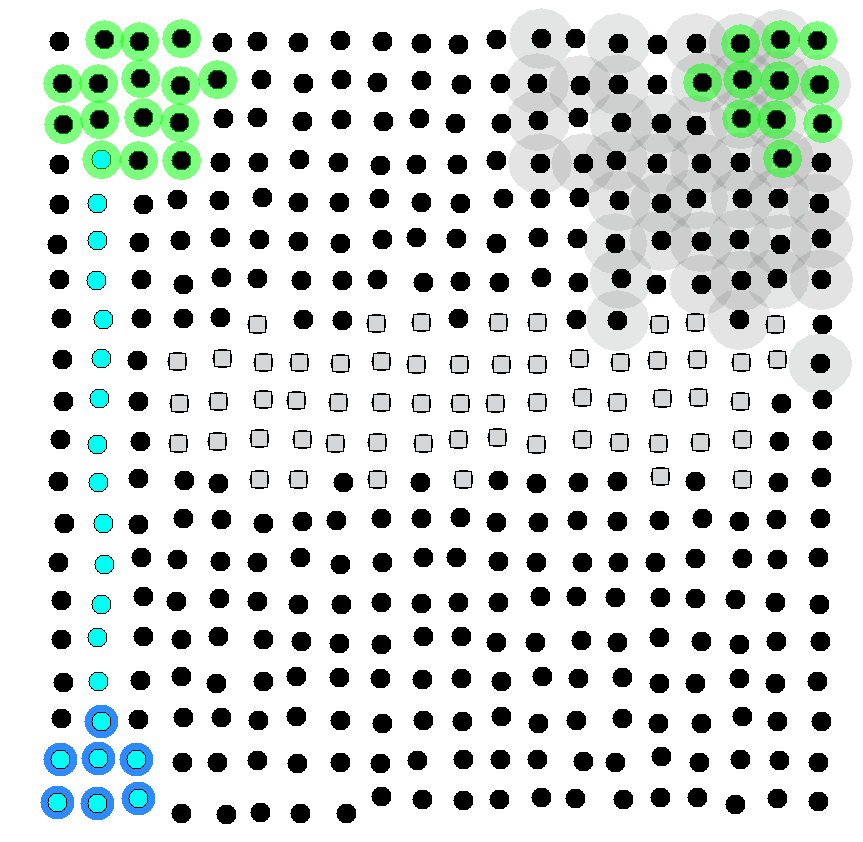
\includegraphics[width=\textwidth]{papers/acsos2023-frp/imgs/channel270.0.png}
      \caption{}
      \label{acsos2023-frp:fig:finish}
  \end{subfigure}\hfill
  \begin{subfigure}[b]{\linewidth}
    \centering
    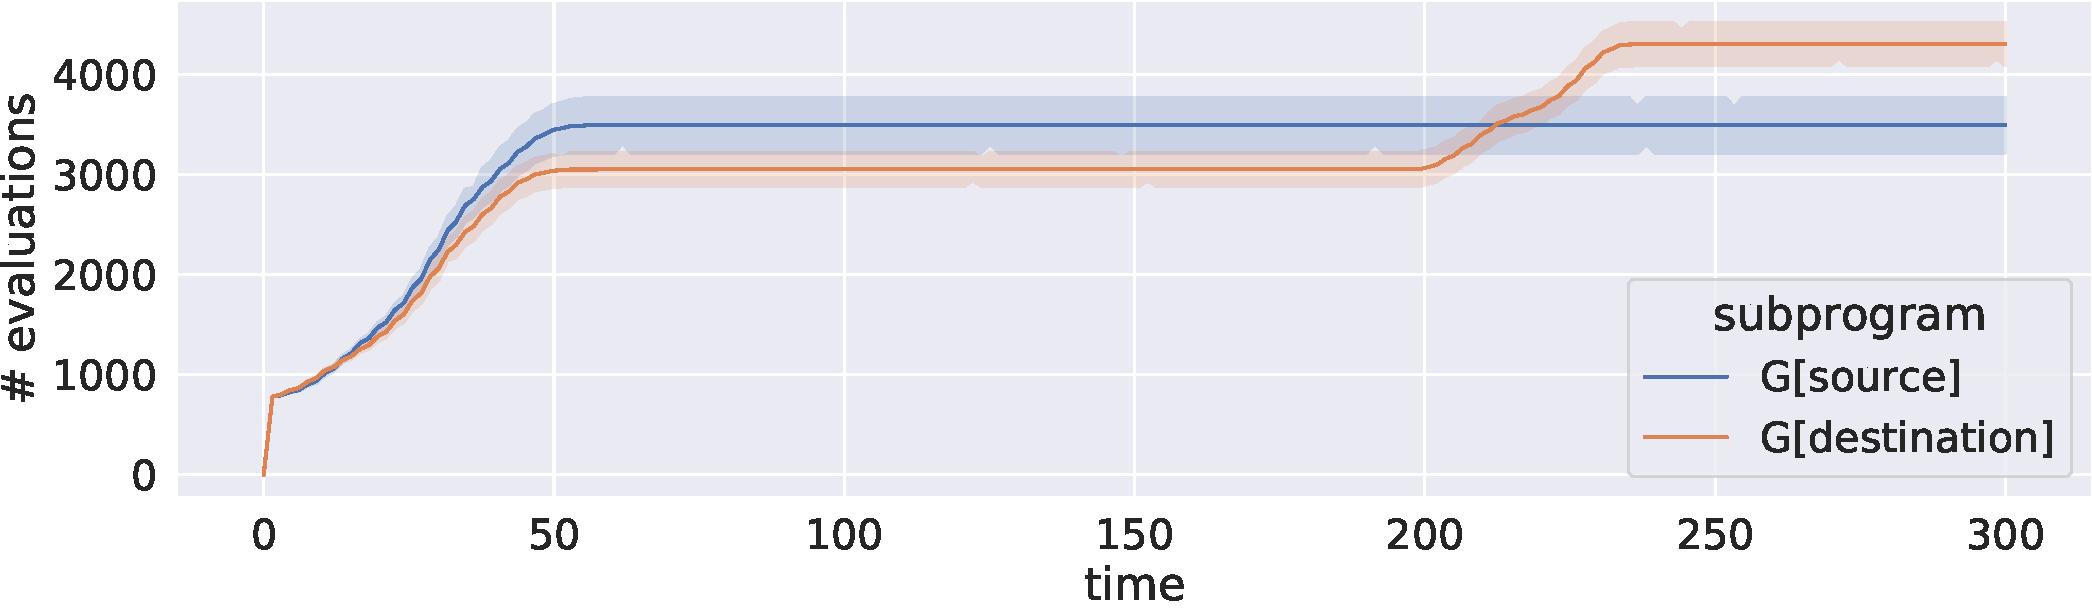
\includegraphics[width=\textwidth]{papers/acsos2023-frp/imgs/message_count.pdf}
  \end{subfigure}
  \caption[behaviour of the channel in response to changes in a destination]{
  The behaviour of the channel in response to changes in a destination is shown through a sequence of snapshots in the first line (using the same graphical notation as \Cref{acsos2023-frp:fig:scenario-screenshots} where, additionally, the grey shadows denote nodes where computation is taking place). 
  It is observed that the computation ``moves'' to different portions of the system until it reaches a stable situation. 
  However, the computation only results in the re-computation of the destination gradient, as seen in the bottom plot.
  }
  \label{acsos2023-frp:fig:subprogram-eval}
\end{figure*}

\section{Wrap up}
\label{acsos2023-frp:sec:conc}

This chapter proposes \ac{langname},
 a \emph{functional reactive macroprogramming model
 for expressing self-organising behaviour}.
%
The language is designed by taking inspiration 
 from the aggregate programming approach,
 which is based on a proactive execution model,
 and reactive approaches to self-organization like TOTA,
 and adopting \ac{frp} as a reference paradigm for its design and implementation.
%
As experimentally verified,
 \ac{langname} allows \emph{tunable, fine-grained reactivity},
 enabling increased communication and time efficiency
 w.r.t. proactive models.
%
Indeed, in \ac{langname},
 a distributed self-organising computation
 turns into a distributed computation dependency graph,
 where distinct sub-computations may execute independently 
 depending on whether their context has changed.

In future work,
 we would like to formalize a core calculus capturing behaviour and properties of \ac{langname} (similarly to field calculi and related formal languages \cite{vbdacp:ac:survey:jlamp,DBLP:conf/ecoop/AudritoCDSV22,DBLP:journals/lmcs/AudritoCDV23}),
 and explore how to support flexibility in actuation models (cf. swarm robotics).
Also, it would be interesting 
  to study the deployment of \ac{langname} applications, e.g.\ by considering how reactive dynamics and consumption profiles may interact with application partitioning strategies like the pulverization model~\cite{CPPVW-FI2020} and deployment options.


%\printbibliography
